        %%******************************************%%
        %%                                          %%
        %%        Modello di tesi di laurea         %%
        %%            di Andrea Giraldin            %%
        %%                                          %%
        %%             2 novembre 2012              %%
        %%                                          %%
        %%******************************************%%


% I seguenti commenti speciali impostano:
% 1. 
% 2. PDFLaTeX come motore di composizione;
% 3. tesi.tex come documento principale;
% 4. il controllo ortografico italiano per l'editor.

% !TEX encoding = UTF-8
% !TEX TS-program = pdflatex
% !TEX root = tesi.tex
% !TEX spellcheck = it-IT
\RequirePackage{filecontents}
\begin{filecontents*}{\jobname.xmpdata}
\Title{Migliorare l'esperienza utente nell'amministrazione della gestione di processo} \Author{Alessio Bettarello}
\Language{it-IT}
\Subject{Tesi di laurea}
\Keywords{gui \sep dashboard \sep gestione di processi \sep process mining \sep front-end}
\end{filecontents*}
\documentclass[10pt,                    % corpo del font principale
               a4paper,                 % carta A4
               twoside,                 % impagina per fronte-retro
               openright,               % inizio capitoli a destra
               english,                 
               italian,                 
               ]{book}    
\PassOptionsToPackage{dvipsnames}{xcolor}
\usepackage[utf8]{inputenc}
\usepackage{colorprofiles}
\usepackage[a-2b,mathxmp]{pdfx}[2018/12/22]
\usepackage[T1]{fontenc}
%**************************************************************
% Importazione package
%************************************************************** 

%\usepackage{amsmath,amssymb,amsthm}    % matematica

\usepackage[T1]{fontenc}                % codifica dei font:
                                        % NOTA BENE! richiede una distribuzione *completa* di LaTeX

\usepackage[utf8]{inputenc}             % codifica di input; anche [latin1] va bene
                                        % NOTA BENE! va accordata con le preferenze dell'editor

\usepackage[english, italian]{babel}    % per scrivere in italiano e in inglese;
                                        % l'ultima lingua (l'italiano) risulta predefinita

\usepackage{bookmark}                   % segnalibri

\usepackage{caption}                    % didascalie

\usepackage{chngpage,calc}              % centra il frontespizio

\usepackage{csquotes}                   % gestisce automaticamente i caratteri (")

\usepackage{emptypage}                  % pagine vuote senza testatina e piede di pagina

\usepackage{epigraph}			% per epigrafi

\usepackage{eurosym}                    % simbolo dell'euro

%\usepackage{indentfirst}               % rientra il primo paragrafo di ogni sezione

\usepackage{graphicx}                   % immagini

\usepackage{hyperref}                   % collegamenti ipertestuali

\usepackage[binding=5mm]{layaureo}      % margini ottimizzati per l'A4; rilegatura di 5 mm

\usepackage{listings}                   % codici

\usepackage{microtype}                  % microtipografia

\usepackage{mparhack,relsize}  % finezze tipografiche

\usepackage{nameref}                    % visualizza nome dei riferimenti                                      

\usepackage[font=small]{quoting}        % citazioni

\usepackage{subfig}                     % sottofigure, sottotabelle

\usepackage[italian]{varioref}          % riferimenti completi della pagina

%\usepackage[dvipsnames]{xcolor}         % colori

\usepackage{booktabs}                   % tabelle                                       
\usepackage{tabularx}                   % tabelle di larghezza prefissata                                    
\usepackage{longtable}                  % tabelle su più pagine                                        
\usepackage{ltxtable}                   % tabelle su più pagine e adattabili in larghezza

\usepackage[toc, acronym]{glossaries}   % glossario
                                        % per includerlo nel documento bisogna:
                                        % 1. compilare una prima volta tesi.tex;
                                        % 2. eseguire: makeindex -s tesi.ist -t tesi.glg -o tesi.gls tesi.glo
                                        % 3. eseguire: makeindex -s tesi.ist -t tesi.alg -o tesi.acr tesi.acn
                                        % 4. compilare due volte tesi.tex.

\usepackage[backend=biber,style=verbose-ibid,hyperref,backref]{biblatex}
                                        % eccellente pacchetto per la bibliografia; 
                                        % produce uno stile di citazione autore-anno; 
                                        % lo stile "numeric-comp" produce riferimenti numerici
                                        % per includerlo nel documento bisogna:
                                        % 1. compilare una prima volta tesi.tex;
                                        % 2. eseguire: biber tesi
                                        % 3. compilare ancora tesi.tex.
                                        \usepackage{float}
                                        \usepackage{color, colortbl}

%**************************************************************
% file contenente le impostazioni della tesi
%**************************************************************

%**************************************************************
% Frontespizio
%**************************************************************

% Autore
\newcommand{\myName}{Alessio Bettarello}                                    
\newcommand{\myTitle}{Migliorare l'esperienza utente nell'amministrazione della gestione di processo}

% Tipo di tesi                   
\newcommand{\myDegree}{Tesi di laurea}

% Università             
\newcommand{\myUni}{Università degli Studi di Padova}

% Facoltà       
\newcommand{\myFaculty}{Corso di Laurea in Informatica}

% Dipartimento
\newcommand{\myDepartment}{Dipartimento di Matematica "Tullio Levi-Civita"}

% Titolo del relatore
\newcommand{\profTitle}{Prof.}

% Relatore
\newcommand{\myProf}{Tullio Vardanega}

% Luogo
\newcommand{\myLocation}{Padova}

% Anno accademico
\newcommand{\myAA}{2019-2020}

% Data discussione
\newcommand{\myTime}{24 Settembre 2020}


%**************************************************************
% Impostazioni di impaginazione
% see: http://wwwcdf.pd.infn.it/AppuntiLinux/a2547.htm
%**************************************************************

\setlength{\parindent}{14pt}   % larghezza rientro della prima riga
\setlength{\parskip}{0pt}   % distanza tra i paragrafi


%**************************************************************
% Impostazioni di biblatex
%**************************************************************
\bibliography{bibliografia} % database di biblatex 

\defbibheading{bibliography} {
    \cleardoublepage
    \phantomsection 
    \addcontentsline{toc}{chapter}{\bibname}
    \chapter*{\bibname\markboth{\bibname}{\bibname}}
}

\setlength\bibitemsep{1.5\itemsep} % spazio tra entry

\DeclareBibliographyCategory{opere}
\DeclareBibliographyCategory{web}

\addtocategory{opere}{womak:lean-thinking}
\addtocategory{web}{site:agile-manifesto}

\defbibheading{opere}{\section*{Riferimenti bibliografici}}
\defbibheading{web}{\section*{Siti Web consultati}}


%**************************************************************
% Impostazioni di caption
%**************************************************************
\captionsetup{
    tableposition=top,
    figureposition=bottom,
    font=small,
    format=hang,
    labelfont=bf
}

%**************************************************************
% Impostazioni di glossaries
%**************************************************************

%**************************************************************
% Acronimi
%**************************************************************
\renewcommand{\acronymname}{Acronimi e abbreviazioni}

\newacronym[description={\glslink{RnDg}{Research and Development}}]
    {rnd}{RND}{Research and development}

\newacronym[description={\glslink{umlg}{Unified Modeling Language}}]
    {uml}{UML}{Unified Modeling Language}

\newacronym[description={\glslink{awsg}{Amazon Web Services}}]{aws}{AWS}{Amazon Web Services}

\newacronym[description={Machine Learning - Apprendimento automatico}]{ml}{ML}{Machine Learning}

\newacronym[description={\glslink{vpng}{Virtual Private Network}}]{vpn}{VPN}{Virtual Private Network}
\newacronym[description={\glslink{kpig}{Key Performance Indicator}}]{kpi}{KPI}{Key Performance Indicator}
\newacronym[description={\glslink{jvmg}{Java Virtual Machine}}]{jvm}{JVM}{Java Virtual Machine}
\newacronym[description={\glslink{uxg}{User Experience}}]{ux}{UX}{User Eperience}
\newacronym[description={\glslink{apig}{Application programming interface}}]{api}{API}{Application Programming Interface}
\newacronym[description={\glslink{ideg}{Integrated Development Environment}}]{ide}{IDE}{Integrated Development Environment}

%**************************************************************
% Glossario
%**************************************************************
\renewcommand{\glossaryname}{Glossario}

\newglossaryentry{RnDg}
{
    name=\glslink{rnd}{R\&D},
    text=Research and development
    sort=red,
    description={in informatica con il termine \emph{Application Programming Interface API} (ing. interfaccia di programmazione di un'applicazione) si indica ogni insieme di procedure disponibili al programmatore, di solito raggruppate a formare un set di strumenti specifici per l'espletamento di un determinato compito all'interno di un certo programma. La finalità è ottenere un'astrazione, di solito tra l'hardware e il programmatore o tra software a basso e quello ad alto livello semplificando così il lavoro di programmazione}
}

\newglossaryentry{umlg}
{
    name=\glslink{uml}{UML},
    text=UML,
    sort=uml,
    description={in ingegneria del software \emph{UML, Unified Modeling Language} (ing. linguaggio di modellazione unificato) è un linguaggio di modellazione e specifica basato sul paradigma object-oriented. L'\emph{UML} svolge un'importantissima funzione di ``lingua franca'' nella comunità della progettazione e programmazione a oggetti. Gran parte della letteratura di settore usa tale linguaggio per descrivere soluzioni analitiche e progettuali in modo sintetico e comprensibile a un vasto pubblico}
}

\newglossaryentry{scrum}
{
    name=SCRUM,
    text=SCRUM,
    sort=scrum,
    description={
    scrum è un framework di metodologie...
    }
}

\newglossaryentry{trello}{
    name=Trello,
    text=Trello,
    sort=trello,
    description={
        Trello è uno strumento di gesitione di progetto...
    }
}

\newglossaryentry{evernote}{
    name=Evernote,
    text=Evernote,
    sort=evernote,
    description={
        Evernote è uno strumento di scrittura collaborativa ...
    }
}

\newglossaryentry{sagemaker}{
    name=SageMaker,
    text=SageMaker,
    sort=sagemaker,
    description={
        SageMaker è un servizio \acrshort{aws}
    }
}

\newglossaryentry{awsg}{
    name=\acrshort{aws},
    text=AWS,
    sort=amazon web services,
    description={
        Gli Amazon Web Services sono ...
    }
}

\newglossaryentry{gitlab}{
    name=GitLab,
    text=GitLab,
    sort=gitlab,
    description={
        GitLab è un servizio di versionamento ...
    }
}
\newglossaryentry{vpng}{
    name=\acrshort{vpn},
    text=VPN,
    sort=virtual private network,
    description={
        Una VPN è una rete ...
    }
}

\newglossaryentry{kpig}{
    name=\acrshort{kpi},
    text=KPI,
    sort=key performance indicator,
    description={
        I Key Performance Indicator sono degli indici ...
    }
}

\newglossaryentry{jvmg}{
    name=\acrshort{jvm},
    text=JVM,
    sort=java virtual machine,
    description={
        La java virtual machine è ..
    }
}

\newglossaryentry{uxg}{
    name=\acrshort{ux},
    text=UX,
    sort=user experience,
    description={
        La User experience ...
    }
}
\newglossaryentry{apig}{
    name=\acrshort{api},
    text=API,
    sort=application programming interface,
    description={
        Per application programming interface si intende ...
    }
}
\newglossaryentry{fork}{
    name=fork,
    text=fork,
    sort=fork,
    description={
        Nell'ambito della gestione delle versioni, una fork è un operazione....
    }
}
\newglossaryentry{ideg}{
    name=IDE,
    text=IDE,
    sort=integrated development environment,
    description={
        Un ambiente di sviluppo integrato è ...
    }
} % database di termini
\makeglossary


%**************************************************************
% Impostazioni di graphicx
%**************************************************************
\graphicspath{{immagini/}} % cartella dove sono riposte le immagini


%**************************************************************
% Impostazioni di hyperref
%**************************************************************
\hypersetup{
    %hyperfootnotes=false,
    %pdfpagelabels,
    %draft,	% = elimina tutti i link (utile per stampe in bianco e nero)
    colorlinks=true,
    linktocpage=true,
    pdfstartpage=1,
    pdfstartview=,
    % decommenta la riga seguente per avere link in nero (per esempio per la stampa in bianco e nero)
    %colorlinks=false, linktocpage=false, pdfborder={0 0 0}, pdfstartpage=1, pdfstartview=FitV,
    breaklinks=true,
    pdfpagemode=UseNone,
    pageanchor=true,
    pdfpagemode=UseOutlines,
    plainpages=false,
    bookmarksnumbered,
    bookmarksopen=true,
    bookmarksopenlevel=1,
    hypertexnames=true,
    pdfhighlight=/O,
    %nesting=true,
    %frenchlinks,
    urlcolor=webbrown,
    linkcolor=RoyalBlue,
    citecolor=webgreen,
    %pagecolor=RoyalBlue,
    %urlcolor=Black, linkcolor=Black, citecolor=Black, %pagecolor=Black
}

%**************************************************************
% Impostazioni di itemize
%**************************************************************
\renewcommand{\labelitemi}{$\ast$}

%\renewcommand{\labelitemi}{$\bullet$}
%\renewcommand{\labelitemii}{$\cdot$}
%\renewcommand{\labelitemiii}{$\diamond$}
%\renewcommand{\labelitemiv}{$\ast$}


%**************************************************************
% Impostazioni di listings
%**************************************************************
\lstset{
    language=[LaTeX]Tex,%C++,
    keywordstyle=\color{RoyalBlue}, %\bfseries,
    basicstyle=\small\ttfamily,
    %identifierstyle=\color{NavyBlue},
    commentstyle=\color{Green}\ttfamily,
    stringstyle=\rmfamily,
    numbers=none, %left,%
    numberstyle=\scriptsize, %\tiny
    stepnumber=5,
    numbersep=8pt,
    showstringspaces=false,
    breaklines=true,
    frameround=ftff,
    frame=single
} 


%**************************************************************
% Impostazioni di xcolor
%**************************************************************
\definecolor{webgreen}{rgb}{0,.5,0}
\definecolor{webbrown}{rgb}{.6,0,0}


%**************************************************************
% Altro
%**************************************************************

\newcommand{\omissis}{[\dots\negthinspace]} % produce [...]

% eccezioni all'algoritmo di sillabazione
\hyphenation
{
    ma-cro-istru-zio-ne
    gi-ral-din
}

\newcommand{\sectionname}{sezione}
\addto\captionsitalian{\renewcommand{\figurename}{Figura}
                       \renewcommand{\tablename}{Tabella}}

\newcommand{\glsfirstoccur}{\ap{{[g]}}}

\newcommand{\intro}[1]{\emph{\textsf{#1}}}

%**************************************************************
% Environment per ``rischi''
%**************************************************************
\newcounter{riskcounter}                % define a counter
\setcounter{riskcounter}{0}             % set the counter to some initial value

%%%% Parameters
% #1: Title
\newenvironment{risk}[1]{
    \refstepcounter{riskcounter}        % increment counter
    \par \noindent                      % start new paragraph
    \textbf{\arabic{riskcounter}. #1}   % display the title before the 
                                        % content of the environment is displayed 
}{
    \par\medskip
}

\newcommand{\riskname}{Rischio}

\newcommand{\riskdescription}[1]{\textbf{\\Descrizione:} #1.}

\newcommand{\risksolution}[1]{\textbf{\\Soluzione:} #1.}

%**************************************************************
% Environment per ``use case''
%**************************************************************
\newcounter{usecasecounter}             % define a counter
\setcounter{usecasecounter}{0}          % set the counter to some initial value

%%%% Parameters
% #1: ID
% #2: Nome
\newenvironment{usecase}[2]{
    \renewcommand{\theusecasecounter}{\usecasename #1}  % this is where the display of 
                                                        % the counter is overwritten/modified
    \refstepcounter{usecasecounter}             % increment counter
    \vspace{10pt}
    \par \noindent                              % start new paragraph
    {\large \textbf{\usecasename #1: #2}}       % display the title before the 
                                                % content of the environment is displayed 
    \medskip
}{
    \medskip
}

\newcommand{\usecasename}{UC}

\newcommand{\usecaseactors}[1]{\textbf{\\Attori Principali:} #1. \vspace{4pt}}
\newcommand{\usecasepre}[1]{\textbf{\\Precondizioni:} #1. \vspace{4pt}}
\newcommand{\usecasedesc}[1]{\textbf{\\Descrizione:} #1. \vspace{4pt}}
\newcommand{\usecasepost}[1]{\textbf{\\Postcondizioni:} #1. \vspace{4pt}}
\newcommand{\usecasealt}[1]{\textbf{\\Scenario Alternativo:} #1. \vspace{4pt}}

%**************************************************************
% Environment per ``namespace description''
%**************************************************************

\newenvironment{namespacedesc}{
    \vspace{10pt}
    \par \noindent                              % start new paragraph
    \begin{description} 
}{
    \end{description}
    \medskip
}

\newcommand{\classdesc}[2]{\item[\textbf{#1:}] #2}
                     % file con le impostazioni personali

\begin{document}
%**************************************************************
% Materiale iniziale
%**************************************************************
\frontmatter
% !TEX encoding = UTF-8
% !TEX TS-program = pdflatex
% !TEX root = ../tesi.tex

%**************************************************************
% Frontespizio 
%**************************************************************
\begin{titlepage}

\begin{center}

\begin{LARGE}
\textbf{\myUni}\\
\end{LARGE}

\vspace{10pt}

\begin{Large}
\textsc{\myDepartment}\\
\end{Large}

\vspace{10pt}

\begin{large}
\textsc{\myFaculty}\\
\end{large}

\vspace{30pt}
\begin{figure}[htbp]
\begin{center}
\includegraphics[height=6cm]{logo-unipd}
\end{center}
\end{figure}
\vspace{30pt} 

\begin{LARGE}
\begin{center}
\textbf{\myTitle}\\
\end{center}
\end{LARGE}

\vspace{10pt} 

\begin{large}
\textsl{\myDegree}\\
\end{large}
\vspace{15pt}
\begin{large}
\textsl{\myTime}
\end{large}

\vspace{40pt} 

\begin{large}
\begin{flushleft}
\textit{Relatore}\\ 
\vspace{5pt} 
\profTitle \myProf
\end{flushleft}

\vspace{0pt} 

\begin{flushright}
\textit{Laureando}\\ 
\vspace{5pt} 
\myName
\end{flushright}
\end{large}

\vspace{40pt}

\line(1, 0){338} \\
\begin{normalsize}
\textsc{Anno Accademico \myAA}
\end{normalsize}

\end{center}
\end{titlepage} 
\input{inizio-fine/colophon}
% !TEX encoding = UTF-8
% !TEX TS-program = pdflatex
% !TEX root = ../tesi.tex

%**************************************************************
% Dedica
%**************************************************************
\cleardoublepage
\phantomsection
\thispagestyle{empty}
\pdfbookmark{Dedica}{Dedica}

\vspace*{3cm}

\begin{center}
    
\end{center}

\medskip

\begin{center}

\end{center}

% !TEX encoding = UTF-8
% !TEX TS-program = pdflatex
% !TEX root = ../tesi.tex

%**************************************************************
% Sommario
%**************************************************************
\cleardoublepage
\phantomsection
\pdfbookmark{Sommario}{Sommario}
\begingroup
\let\clearpage\relax
\let\cleardoublepage\relax
\let\cleardoublepage\relax

%**************************************************************
\chapter*{Presentazione dell'elaborato}
\begin{description}
    \item[{\hyperref[cap:introduzione]{Il primo capitolo}}] presenta il contesto aziendale nel quale ho svolto l'attività di stage
    \item[{\hyperref[cap:process-mining]{Il secondo capitolo}}] descrive da dove nasce l'esigenza di monitorare e gestire processi tramite l'impiego di software
    
    \item[{\hyperref[cap:modalita-svolgimento]{Il terzo capitolo}}] approfondisce le metodologie e il prodotto software oggetto di stage
    
    \item[{\hyperref[cap:performance-stage]{Il quarto capitolo}}] mostra come l'esperienza di stage ha influito sullo studente
    
\end{description}

Riguardo la stesura del testo, relativamente al documento sono state adottate le seguenti convenzioni tipografiche:
\begin{itemize}
	\item gli acronimi, le abbreviazioni e i termini ambigui o di uso non comune menzionati vengono definiti nel glossario, situato alla fine del presente documento;
	\item per la prima occorrenza dei termini riportati nel glossario viene utilizzata la seguente nomenclatura: \emph{parola}\glsfirstoccur;
	\item i termini in lingua straniera o facenti parti del gergo tecnico sono evidenziati con il carattere \emph{corsivo};
\end{itemize}


%\vfill
%
%\selectlanguage{english}
%\pdfbookmark{Abstract}{Abstract}
%\chapter*{Abstract}
%
%\selectlanguage{italian}

\endgroup			

\vfill


% !TEX encoding = UTF-8
% !TEX TS-program = pdflatex
% !TEX root = ../tesi.tex

%**************************************************************
% Ringraziamenti
%**************************************************************
\cleardoublepage
\phantomsection
\pdfbookmark{Ringraziamenti}{ringraziamenti}



\bigskip

\begingroup
\let\clearpage\relax
\let\cleardoublepage\relax
\let\cleardoublepage\relax

\chapter*{Ringraziamenti}

\noindent\textit{\myLocation, \myTime}
\hfill \myName

\endgroup


% !TEX encoding = UTF-8
% !TEX TS-program = pdflatex
% !TEX root = ../tesi.tex

%**************************************************************
% Indici
%**************************************************************
\cleardoublepage
\pdfbookmark{\contentsname}{tableofcontents}
\setcounter{tocdepth}{2}
\tableofcontents
%\markboth{\contentsname}{\contentsname} 
\clearpage

\begingroup 
    \let\clearpage\relax
    \let\cleardoublepage\relax
    \let\cleardoublepage\relax
    %*******************************************************
    % Elenco delle figure
    %*******************************************************    
    \phantomsection
    \pdfbookmark{\listfigurename}{lof}
    \listoffigures

    %\vspace*{8ex}
    \newpage
    %*******************************************************
    % Elenco delle tabelle
    %*******************************************************
    \phantomsection
    \pdfbookmark{\listtablename}{lot}
    \listoftables
        
    \vspace*{8ex}
\endgroup

\cleardoublepage

\cleardoublepage

%**************************************************************
% Materiale principale
%**************************************************************
\mainmatter
% !TEX encoding = UTF-8
% !TEX TS-program = pdflatex
% !TEX root = ../tesi.tex

%**************************************************************
\chapter{Introduzione}
\label{cap:introduzione}
%**************************************************************
\section{La realtà Siav S.p.a.}

Presentazione di massima dell'azienda Siav contenente ambiti di sviluppo, reparti e divisioni

%**************************************************************
\section{Il reparto ricerca e sviluppo}

Presentazione del mio reparto, di cosa si occupa, che tipologie di attività effettua
%**************************************************************
\subsection{Il way of working del reparto}
Spiegazione delle tecnologie e processi in uso in reparto

%**************************************************************
\subsection{Formazione continua}
Spiego come frequenti sessioni di formazione ( nel particolare del periodo in cui ero impiegato in siav, principalmente sui servizi AWS) portano il reparto a saper riconoscere e discutere al meglio delle soluzioni per ogni problema che si pone di risolvere.

%**************************************************************
\section{Produzione tramite sperimentazione}
Presentazione della filosofia che muove le molteplici attività i stage che Siav effettua in collaborazione con le università e come essa porti valore aggiunto al prodotti stesso.
Presentazione del concept software "Bipod", di chi ne è il proponente e da cosa è composto.
Spiegazione del perché la natura di Bipod è sperimentale (ovvero perché argomento di diversi stage)
%**************************************************************
             % Introduzione
% !TEX encoding = UTF-8
% !TEX TS-program = pdflatex
% !TEX root = ../tesi.tex

%**************************************************************
\chapter{Il contesto del process mining}
\label{cap:process-mining}
%**************************************************************

\intro{Brevissima introduzione al capitolo}\\

%**************************************************************
\section{La gestione dei processi aziendali}
Spiega l'origine della necessità di gestire e monitorare i processi
%**************************************************************
\section{Da dato ad informazione}
Spiega l'importanza del passaggio da dato ad informazione introducendo il concetto di kpi e il perché sia altrettanto importante agevolarne quanto più possibile la creazione
%**************************************************************
\section{Kpi e dashboards nel process mining}
Introduce il concetto di dashboard, spiega perché dashboard e kpi aiutino l'attività di monitoraggio e verifica delle prestazioni 

%**************************************************************
\section{I ruoli nella gestione e amministrazione di processo}

Definisce i ruoli che sfruttano la piattaforma e l'utilità che percepiscono dal suo uso

%**************************************************************             % Il contesto del process mining
% !TEX encoding = UTF-8
% !TEX TS-program = pdflatex
% !TEX root = ../tesi.tex

%**************************************************************
\chapter{Svolgimento del progetto}
\label{cap:modalita-svolgimento}
%**************************************************************
\section{Aspettative del progetto}
\label{sec:aspettative}
Nei primi giorni di stage ho individuato i requisiti che la piattaforma avrebbe dovuto soddisfare per portare a termine gli obiettivi.
Le funzionalità che dovevo implementare in Bipod si concretizzano nei requisiti individuati dal codice nel formato:
\begin{center}
    \noindent R<tipo><progressivo> - <descrizione>
\end{center}
dove:
\begin{itemize}
    \item tipo identifica la tipologia in base agli obiettivi cui deve adempiere:
    \begin{itemize}
        \item \textbf{O} - Obbligatorio;
        \item \textbf{F} - Facoltativo;
    \end{itemize}
    \item Progressivo è un codice composto da più numeri separati dal carattere "." che indicano il rapporto gerarchico fra i requisiti.
\end{itemize}
I seguenti requisiti sono quelli principali:
\begin{longtable}[!h]{|p{0.2\textwidth}|p{0.8\textwidth}|}
    \hline
        \textbf{Codice} & \textbf{Requisito} \\ \hline
         RO1 & Gestione autenticazione \\ \hline
         RO2 & Gestione e inserimento \acrshort{kpi} \\ \hline
         RO2.1 & Selezione del processo\\ \hline
         RO2.2 & Inserimento e gestione termini\\ \hline
         RO2.2.1 & Inserimento filtri di ricerca\\ \hline
         RO2.2.2 & Selezione tipologia operazione\\ \hline
         RO2.2.3 & Selezione intervallo temporale\\ \hline
         RO2.3 & Inserimento formula e soglie per il \acrshort{kpi}\\ \hline
         RO3 & Vista elenco \acrshort{kpi}\\ \hline
         RO3.1 & Filtraggio entry\\ \hline
         RO3.2 & Selezione della modalità di visualizzazione\\ \hline
         RO3.3 & Modifica e cancellazione di \acrshort{kpi}\\ \hline
         RF1 & Vista e gestione \textit{dashboard}\\ \hline
         RF1.1 & Configurazione delle componenti \textit{dashboard}\\ \hline
         RF1.1.1 & Selezione di un particolare tipo di componente grafico\\ \hline
         RF1.1.2 & Selezione della \acrshort{kpi} che il componente deve rispecchiare\\ \hline
         RF1.1.3 & Selezione della posizione del componente grafico\\ \hline
         RF1.1.4 & Selezione della dimensione del componente grafico\\ \hline
         RF2 & Configurazione \textit{dashboard} per amministratore\\ \hline
         RF3 & Vista grafo di processo\\ \hline
         RF3.1 & Selezione del processo di riferimento\\ \hline
         RF3.2 & Visualizzazione dettaglio eventi all'interno dei nodi\\ \hline
         RF3.3 & Visualizzazione dettaglio temporale al passaggio sugli archi\\ \hline
    \caption{Elenco principali requisiti funzionali}
    \label{tab:requirements}
\end{longtable}
\section{Metodo di sviluppo}
%**************************************************************
\subsection{L'uso di cicli di sviluppo}
Il progetto di stage iniziale prevedeva un ciclo unico di sviluppo. Esso comprendeva delle attività di formazione individuale seguite dalle attività di analisi, progettazione, implementazione e verifica.
Rispetto al progetto iniziale di restaurare il prototipo che era stato sviluppato dal \textit{team} per testare le funzionalità \textit{back-end}, ho proposto di effettuare un approfondita analisi incentrata sull'esperienza utente. Questo perché avevo notato la completa assenza di strutturazione, la presenza di codice non utile allo scopo della piattaforma e povero di separazione. Erano caratteristiche comprensibili derivanti dalla sua natura prototipale ma non accettabili in un prodotto manutenibile e incrementabile.
Durante l'attività di analisi, il responsabile, si è reso subito conto che la profondità con cui la stavo effettuando avrebbe potuto introdurre diverse insidie comportanti la responsabilità di prendere delle scelte importanti per il destino della piattaforma.

In accordo con il tutor, abbiamo deciso di sezionare il progetto in diversi cicli di sviluppo, uno per funzionalità. Questi hanno infatti introdotto un numero superiore di momenti di verifica permettendo di lavorare con maggiore efficacia, puntando sempre alla giusta meta.
Per ognuna delle funzionalità individuate, assieme al responsabile, abbiamo programmato un ciclo di sviluppo che comprendeva, oltre che le attività previste per il ciclo iniziale, quella di raffinamento dei requisiti già individuati.

%**************************************************************
\subsection{Diagrammi e formalizzazione}
\label{ssec:diagrams}
Per eliminare l'insorgere di ambiguità, ho deciso di effettuare l'attività di analisi con estrema minuziosità e completezza.
Sono partito dalla gestione degli accessi alla piattaforma, ho affrontato la visualizzazione dei grafi di processo, passando poi alla visualizzazione dei \acrshort{kpi}, al loro editing e infine alla gestione delle \textit{dashboard}.
Per donare completezza al documento prodotto dall'attività, ho preferito schematizzare, tramite i diagrammi dei casi d'uso, tutti gli scenari che l'utente può affrontare all'interno della piattaforma.

I casi d'uso, assieme ai rispettivi diagrammi, costituiscono l'espressione più formale e precisa possibile dell'\acrshort{ux} in quanto esprimono tutte le interazioni che l'utente ha la possibilità di fare in base alle sue necessità.
%**************************************************************
\subsection{Confronto continuo}
La chiave di successo che ha maggiormente contribuito al raggiungimento degli obiettivi, è stata la frequenza di verifica della progressione e della direzione intrapresa dal progetto.

Durante l'attività di analisi, il confronto continuo con responsabile e tutor, ha permesso di individuare i requisiti con precisione, facendo subito emergere lacune nella mia preparazione sull'argomento \textit{process mining}.

Per quanto concerne il \textit{design}, verificare periodicamente le modalità di interazione ha dato al responsabile l'opportunità di toccare con mano le mie idee a livello di \acrshort{ux}.

Durante l'implementazione, la collaborazione con il tutor tramite frequenti confronti, ha permesso che le esigenze che avevo espresso a livello \textit{front-end}, trovassero riscontro nella partizione \textit{back-end}.

Fondamentale è stata anche la presenza di tutti durante questi momenti di verifica: il tutor, analisi alla mano, verificava la correttezza, il responsabile forniva un parere esterno e perciò più critico.
Inoltre, nel caso di dubbi, le proposte venivano vagliate più velocemente discutendo la strada da percorrere e registrando le decisioni in un documento condiviso.

%**************************************************************
\subsection{\acrlong{poc}}
Durante la progettazione dell'interfaccia, il responsabile, mi ha chiesto di realizzare dei \textit{mock-up} della stessa per verificarne prontamente la correttezza.
Tutor e responsabile, mi hanno lasciato la libertà di scegliere tra due software di progettazione: Balsamiq Wireframe e Figma. Entrambi sono valide alternative ma per il secondo sono state sviluppate delle librerie che includono le componenti Material Design.
Ho cominciato prima a formarmi sul funzionamento di Figma. Dopo aver fatto qualche prova, ho prodotto il primo \textit{mock-up}. Responsabile e tutor si sono accorti che, visto che ormai avevo preso una certa dimestichezza con Angular e Material Design durante la formazione iniziale, il tempo impiegato per creare \textit{mock-up} era troppo alto rispetto alla velocità di realizzazione di \acrshort{poc}\glsfirstoccur che dimostrassero ciò che era stato trattato nell'analisi dei requisiti. Inoltre, tramite la corretta strutturazione del codice, le modifiche risultavano estremamente veloci da fare tramite interventi sui \textit{template} dei \textit{component}.
Queste due constatazioni hanno portato alla scelta di evitare la progettazione in modalità grafica quando possibile a favore di una più completa dimostrazione dell'usabilità tramite la realizzazione di \acrlong{poc} per ogni funzionalità.

Ho cominciato perciò con la definizione del \textit{service} per la comunicazione con il \textit{back-end}. Dopodiché, ne ho effettuato un \textit{mock-up} in attesa degli interventi di correzione che andavano effettuati all'interno della partizione \textit{log-uploader}.

Tale \textit{mock-up} è stato poi impiegato durante la progettazione di tutte le rimanenti interfacce.
\newpage
%**************************************************************
\subsection{Documentazione ampia e prolissa}
Durante tutte le attività svolte per il progetto, ho cercato di documentare più dettagli possibili.
In particolare:
\begin{itemize}
    \item I casi d'uso riportano sia lo scenario, sia il dettaglio con precondizioni e postcondizioni;
    \item I requisiti individuati sono categorizzati e dettagliati;
    \item Nella documentazione tecnica di progettazione, ho inserito diverse immagini illustranti il funzionamento desiderato della piattaforma, lo scopo della funzionalità descritta e la motivazione di eventuali scelte tecniche intraprese;
    \item Il codice sorgente da me scritto, utilizza nomi estremamente evocativi; \item Ho ampiamente documentato ogni modulo, funzione, modello, servizio o classe, tramite lo standard \gls{jsdoc}\glsfirstoccur non lasciando alcuna porzione scoperta.
\end{itemize}

Nella strategia incrementale che Siav impiega per Bipod, questo è necessario per permettere, a chi effettuerà altri incrementi alla piattaforma, di comprendere velocemente la strutturazione attuale delle componenti e di accelerare perciò l'implementazione degli incrementi stessi.
\vspace{45px}
\begin{figure}[H]
    \centering
    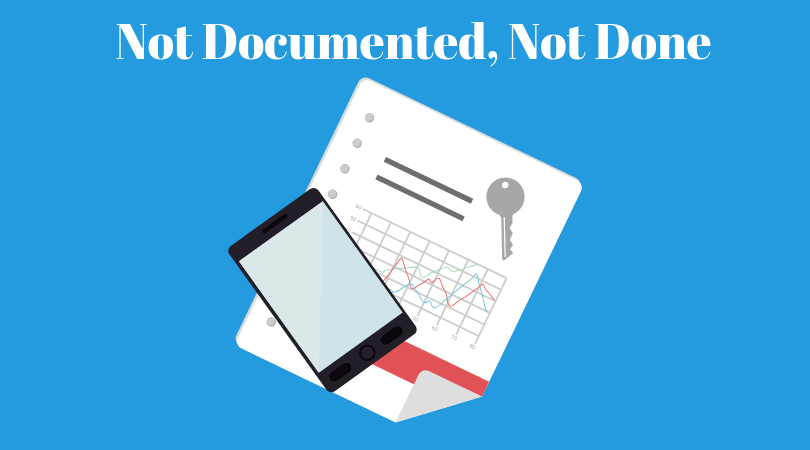
\includegraphics[width=0.75\columnwidth]{immagini/Not-documented-not-done.png}
    \caption{Non documentato = non fatto - Fonte: \href{https://cpahalltalk.com/audit-documentation/}{Audit Documentation - CPA Hall Talk}}
    \label{fig:notDone}
\end{figure}
\newpage
%**************************************************************
\section{Priorità e criticità}
%**************************************************************
\subsection{Tecnologie software sfruttate}
In questa sezione espongo come ho sfruttato alcune tecnologie indicate in \S\ref{ssec:techEnvolved} assieme a quelle introdotte dall'attività di stage e agli strumenti indicati in \S\ref{ssec:usedTools}.
\vspace{40pt}
\begin{figure}[H]
    \centering
    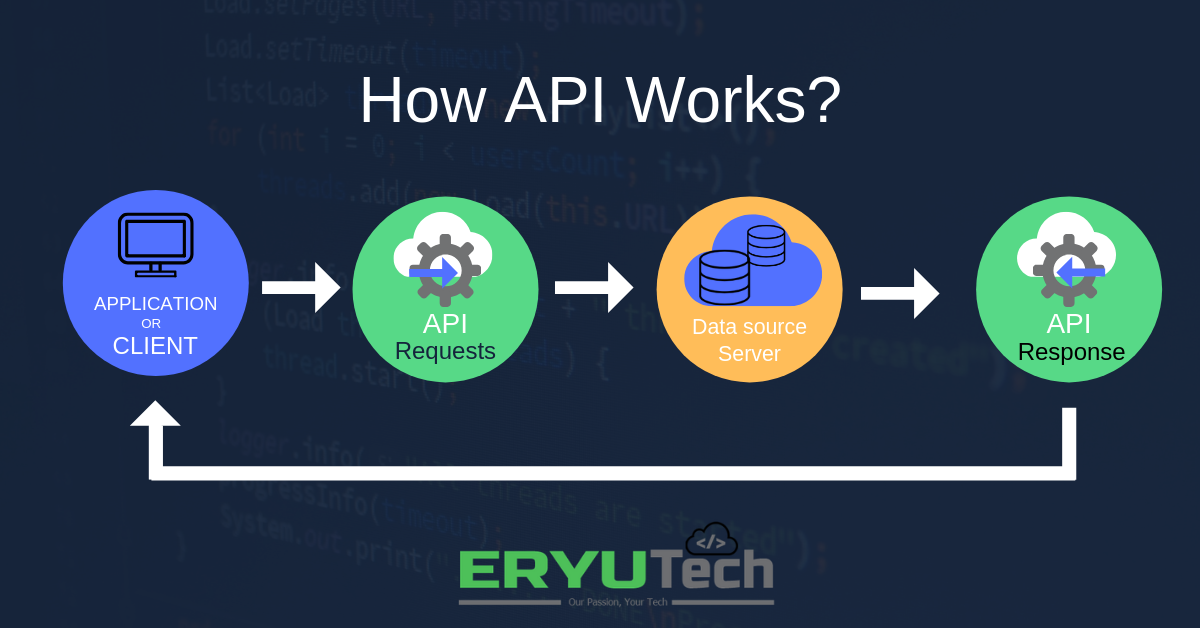
\includegraphics[width=0.9\columnwidth]{immagini/how_api_works.png}
    \caption{Come funzionano le \acrshort{api} - Fonte: \href{https://www.facebook.com/eryutech/photos/application-programming-interface-apihow-it-works-eryutech/1125855790904330/}{ERYUTech}}
    \label{fig:howApiWorks}
\end{figure}
%**************************************************************
\subsubsection{Docker}
\label{ssec:docker}
Questo strumento si basa su \textit{file} di configurazione che permettono la virtualizzazione di vari servizi. Con estrema flessibilità, modificando tali \textit{file}, è possibile modificare la topologia della rete che collega i servizi e le risorse associate agli stessi. All'inizio dell'attività di stage mi è stato fornito un \textit{laptop} per accedere alla rete interna e lavorare così sui \textit{repository} condivisi.

Il reparto, tramite l'intervento dell'amministratore, effettua \acrshort{ci} tramite il \textit{deploy} manuale su un server virtuale interno all'azienda. Per crearmi un ambiente di pseudo integrazione continua, ho preferito virtualizzare l'ambiente di produzione in locale non esistendo alcun tipo di test di integrazione predisposto per il lato back-end. Dopo pochi giorni, è diventato inutilizzabile a causa di scarsità di memoria volatile. Dopo aver identificato il problema nella virtualizzazione dei servizi, ho individuato quali erano quelli essenziali per l'esecuzione della partizione \textit{front-end} e ho scartato dal file di configurazione di Docker, quelli che non venivano sfruttati.
La velocità con cui ho risolto un problema che sembrava molto difficile da risolvere, mi ha fatto capire quanto Docker sia facilmente adattabile ad ogni situazione.
\newpage
%**************************************************************
\subsubsection{Angular}
La potenzialità maggiore derivata dall'impiego di questo \textit{framework} risiede, anche in questo caso, nella flessibilità. Questo perché esso è orientato all'impiego di modelli di dato e di vista: premette perciò di rappresentare facilmente informazioni di diversa origine in maniera dinamica semplicemente cambiando template oppure cambiandone la classe di comportamento associata.
Inoltre va a braccetto con Material Design essendo entrambi sviluppati e manutenuti da Google. L'integrazione della libreria grafica Material mi è risultata estremamente facile ed intuitiva, e perciò lo è anche per i programmatori meno esperti.

Un'altra funzionalità che ho largamente sfruttato è la creazione di file \acrshort{xml} per l'internalizzazione: tramite il comando \verb|ng xi18n|, Angular genera un file nel formato specificato (\acrshort{xliff}\glsfirstoccur 1.2 se non specificato). Questa operazione si basa sulla marchiatura degli elementi localizzabili tramite un apposito attributo (nel caso di codice HTML) o annotazione (nel sorgente TypeScript). L'\textit{output} è un file di lingua \emph{sorgente}. Va generato ogniqualvolta vengano introdotti nuovi elementi testuali specifici della lingua di sviluppo o che comportano utilizzo di variabili che vanno localizzate come importi in valuta o date (di default vengono interpretati come inglese americano) all'interno delle interfacce o del codice. Costruendo traduzioni sulla base di quel \textit{file}, è possibile effettuare una \textit{build} per la località di destinazione passandolo come parametro.
%**************************************************************
\subsubsection{NodeJS}
"Node.js® è un \textit{runtime} JavaScript costruito sul motore JavaScript V8 di Chrome"\footcite{site:nodeJS}. Nel progetto è stato utilizzato per eseguire in locale il servizio \textit{front-end}. Tramite il suo file di configurazione \emph{package.json}, ho definito diverse versioni di \textit{build} che vengono eseguite automaticamente per generare le versioni internazionalizzate della piattaforma.
%**************************************************************
\subsubsection{Nginx}
Come ogni servizio degno di nota, anche Nginx sfrutta un \textit{file} di configurazione per servire le pagine web. Le modifiche che ho effettuato a tale file, sono atte a servire le versioni internazionalizzate tramite prefissi di indirizzo.
%**************************************************************
\subsubsection{Micronaut}
Tramite Micronaut, ho effettuato delle modifiche al codice \textit{back-end} per correggere il mancato rispetto dei principi \acrshort{rest} e collaborare con il tutor all'introduzione delle nuove funzionalità \textit{front-end}. Avevo avuto poca esperienza con le annotazioni nel linguaggio Java ma, documentazione e diversi esempi alla mano, sono riuscito ad alterare le API correggendole dove necessario.

Il \textit{framework} Micronaut è molto vasto per modalità di impiego e opzioni disponibili e ciò si riflette sulla dimensione della documentazione di riferimento.
Una critica che mi permetto di fare è che spesso le informazioni mi sono risultate frammentarie all'interno delle varie sezioni e per recuperare la corretta e completa annotazione utile alla creazione di una \acrshort{api} non basilare, ho dovuto ricorrere alla ricerca di esempi di impiego da fonti esterne.
\begin{figure}[H]
    \centering
    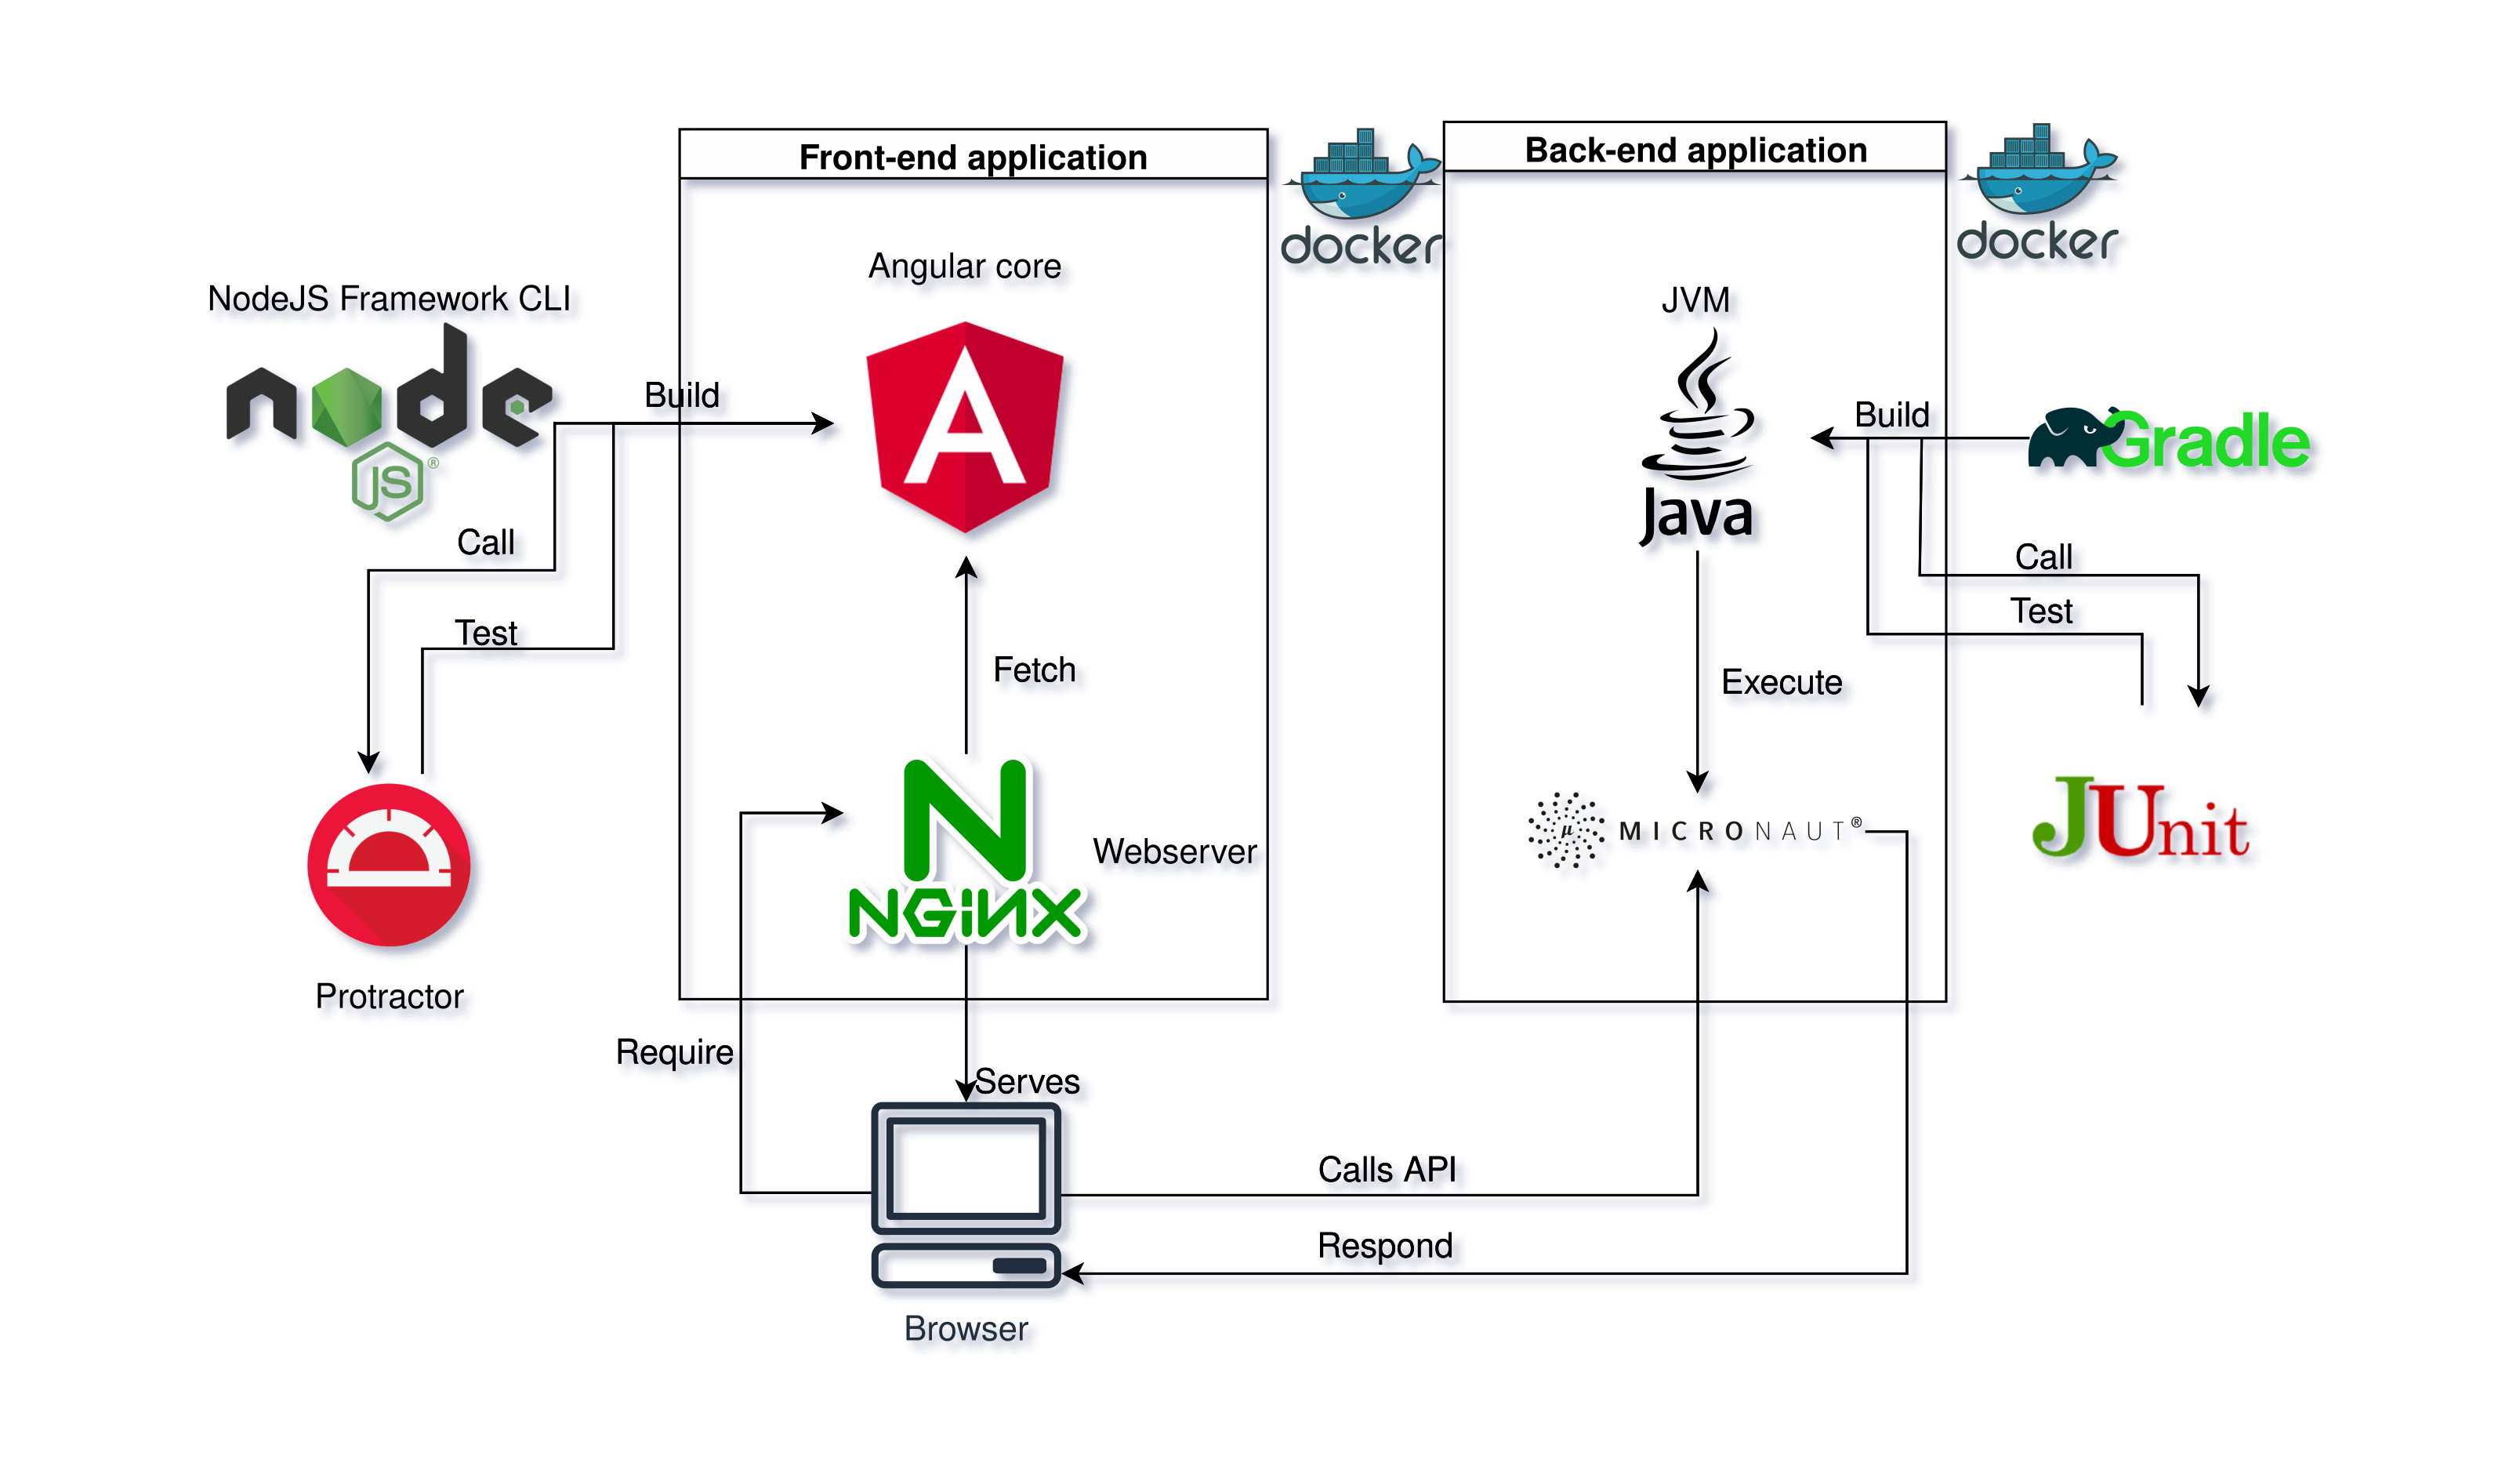
\includegraphics[width=\columnwidth]{immagini/Network scheme-2.png}
    \caption{Interazione fra le tecnologie impiegate}
    \label{fig:techInteraction}
\end{figure}
%**************************************************************
\subsubsection{PoEdit}
Dopo essermi documentato attentamente sul formato \acrshort{xliff}, ho dovuto creare un file di traduzione per mettere in atto ciò che avevo imparato. L'idea iniziale proposta dal tutor era quella di modificare manualmente il file \acrshort{xliff} originale introducendo la traduzione nella lingua \textit{target}. Non ritenendo utile procedere in questa maniera, ho subito pensato che doveva per forza esistere un software che permettesse agevolmente di effettuare questa operazione. La risposta è arrivata consultando \gls{discover}\glsfirstoccur dove ho trovato PoEdit.
Questo \textit{tool} è risultato molto efficace nella creazione di traduzione di \textit{file} in formato \emph{gettext} e \acrshort{xliff}. Utilizzabile anche in connessione al \textit{localization management service} Crowdin. Permette di:
\begin{itemize}
    \item Selezionare una lingua di destinazione;
    \item Passare velocemente da una voce all'altra inserendone la traduzione;
    \item Verificare automaticamente la presenza parziale di tutte le traduzioni;
    \item Verificare automaticamente la coerenza delle traduzioni inserite controllandone la formattazione;
    \item Effettuare le operazioni descritte sopra su un file di \textit{localization} condiviso su Crowdin.
\end{itemize}
\newpage
%**************************************************************
\subsection{Strumenti di collaborazione}
%**************************************************************
\subsubsection{Comunicazione}
Nonostante essa fosse frequente, la comunicazione durante lo stage, non è stata la più semplice delle attività. Sono stati coinvolti troppi strumenti senza mantenere una scelta condivisa. Ho però potuto notare pregi e difetti di tutti quelli che abbiamo impiegato.
\paragraph{Telegram} Lo abbiamo sfruttato principalmente per l'organizzazione degli appuntamenti collettivi tramite la creazione di un gruppo condiviso. \'E stato utile anche ove c'era la necessità di effettuare chiamate fra terminali di diverso tipo (ad esempio da PC a telefono).
Fra le varie caratteristiche, Telegram permette di condividere, con i propri contatti, files di grandi dimensioni\footcite{site:telegram}, funzionalità che in reparto abbiamo ampiamente apprezzato.
%**************************************************************
\paragraph{Zoom} Il \textit{client} di videoconferenze americano ha avuto molto successo durante quest'anno grazie al largo impiego in ambito aziendale e scolastico rientrando nei software indispensabili di molte persone\footcite{site:zoomBlog}. Il pregio che ho potuto rilevare è la bassa sete di banda e di caratteristiche \textit{hardware}. Degne di nota anche la funzione di controllo remoto e la vastità delle opzioni configurabili.
\vspace{30pt}
\begin{figure}[H]
    \centering
    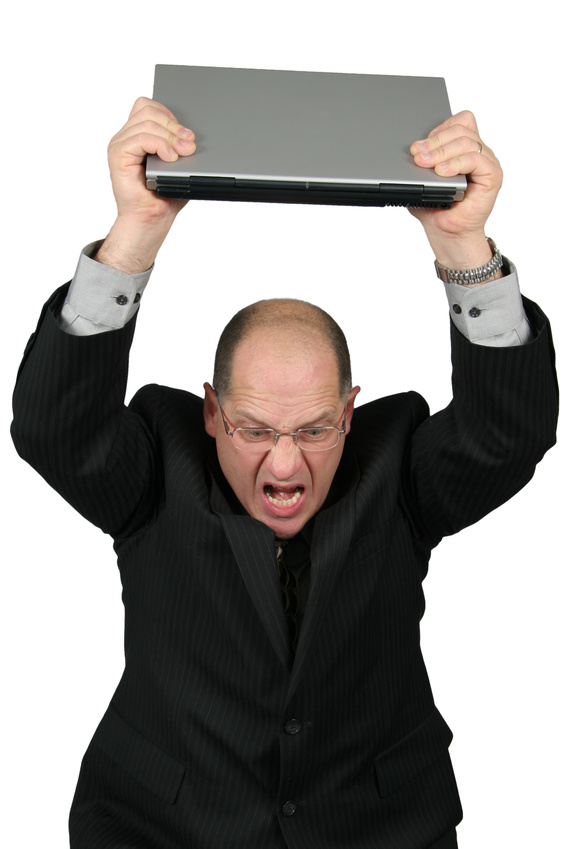
\includegraphics[width=0.35\columnwidth]{immagini/vc_struggle.jpg}
    \caption{\textit{Video call struggle} - Fonte: \href{https://www.commsbusiness.co.uk/news/9-out-of-10-people-struggle-when-connecting-to-a-video-conference-call/}{9 out of 10 people struggle when connecting to a video conference call - Comms Business}}
    \label{fig:vcStruggle}
\end{figure}
\newpage
Non mancano, però evidenti difetti che ho potuto rilevare. Per primo, quello trascurabile dell'interfaccia grafica, poco gradevole e rievocante software datati. Il secondo, un'esperienza utente da dimenticare\footnote{Versione 5.2 su Kubuntu 20.04}:
\begin{itemize}
    \item Accesso alle riunioni macchinoso;
    \item Comportamenti indesiderati frequenti come ingresso in modalità \textit{full-screen} automatico;
    \item Disorientamento causato dalla operatività su molteplici finestre;
    \item Strumenti che passano dall'essere introvabili all'invadenza nella modalità \textit{full-screen};
    \item Passaggio fra account Google diversi estremamente difficile e dedicato solo a esperti informatici;
    \item Limite tempo massimo nelle riunioni nella versione free;
    \item Destinazione delle chiamate private non omogenea: chiamando un contatto potrebbe avviarsi la suoneria su un terminale o sull'altro non considerando lo stato di blocco di uno di quelli.
\end{itemize}
Per le scarse caratteristiche tecniche dell'hardware a mia disposizione, lo prediligo in molti casi alla concorrenza ma non esiterei a scartarlo qualora impiegassi un \textit{device} diverso.
%**************************************************************
\paragraph{MS Teams}
Il \textit{tool} prodotto da Microsoft è nel complesso un buon prodotto: risponde infatti alla maggior parte delle esigenze di comunicazione e condivisione che un gruppo può avere. Unica debolezza riscontrata è che la collaborazione fra \textit{team} di diverse organizzazioni non è agevolata, limitando l'operatività.
Si integra perfettamente nell'ambiente \gls{office} ed è disponibile per molteplici sistemi operativi.
%**************************************************************
\subsubsection{Documentazione}
%**************************************************************
\paragraph{\LaTeX}
Per l'analisi dei requisiti, ho deciso di effettuare la stesura in \LaTeX.
Dal mio punto di vista, risulta più comodo perché, come ad esempio per il linguaggio \gls{markdown}\glsfirstoccur, è più facile da versionare all'interno di un \textit{repository} e da monitorare tramite \gls{diff}\glsfirstoccur.
%**************************************************************
\paragraph{Google Docs}
Il tool offerto da Google permette di creare documenti condivisi in maniera semplice e veloce. Possiede le funzionalità essenziali dei classici \textit{tool} di \textit{office automation}, sufficienti allo scopo. Le funzionalità più interessanti di questo strumento sono lo \textit{storaging} su Google Drive e il registro delle modifiche che tiene traccia di quali editori hanno effettuato determinate modifiche nel tempo.
\newpage
%**************************************************************
\paragraph{Evernote}
Il \textit{tool} (introdotto in \S\ref{ssec:usedTools}) fornisce il vantaggio di condividere velocemente appunti con i colleghi. Molto utile anche la funzionalità di allegazione di documenti pdf alle note, utile quando c'è bisogno di fare delle annotazioni con riferimenti ad uno specifico documento locale. Nell'utilizzo collaborativo, risulta essere un disastro: non è infatti possibile usufruire contemporaneamente dello stesso documento in modalità di modifica. Inoltre, per ragioni non ancora note, durante un accesso accidentalmente sincronizzato, il responsabile ha perso tutti i contenuti grafici allegati alla nota che stava elaborando; comportamento decisamente non desiderabile, anche perché a detta sua, recidivo.

Nonostante io sia stato un utilizzatore dal momento del lancio fino all'arrivo della Google Suite, sostengo che Evernote è in difficoltà per funzionalità e stabilità a competere con i concorrenti.
\vspace{20pt}
\begin{figure}[H]
    \centering
    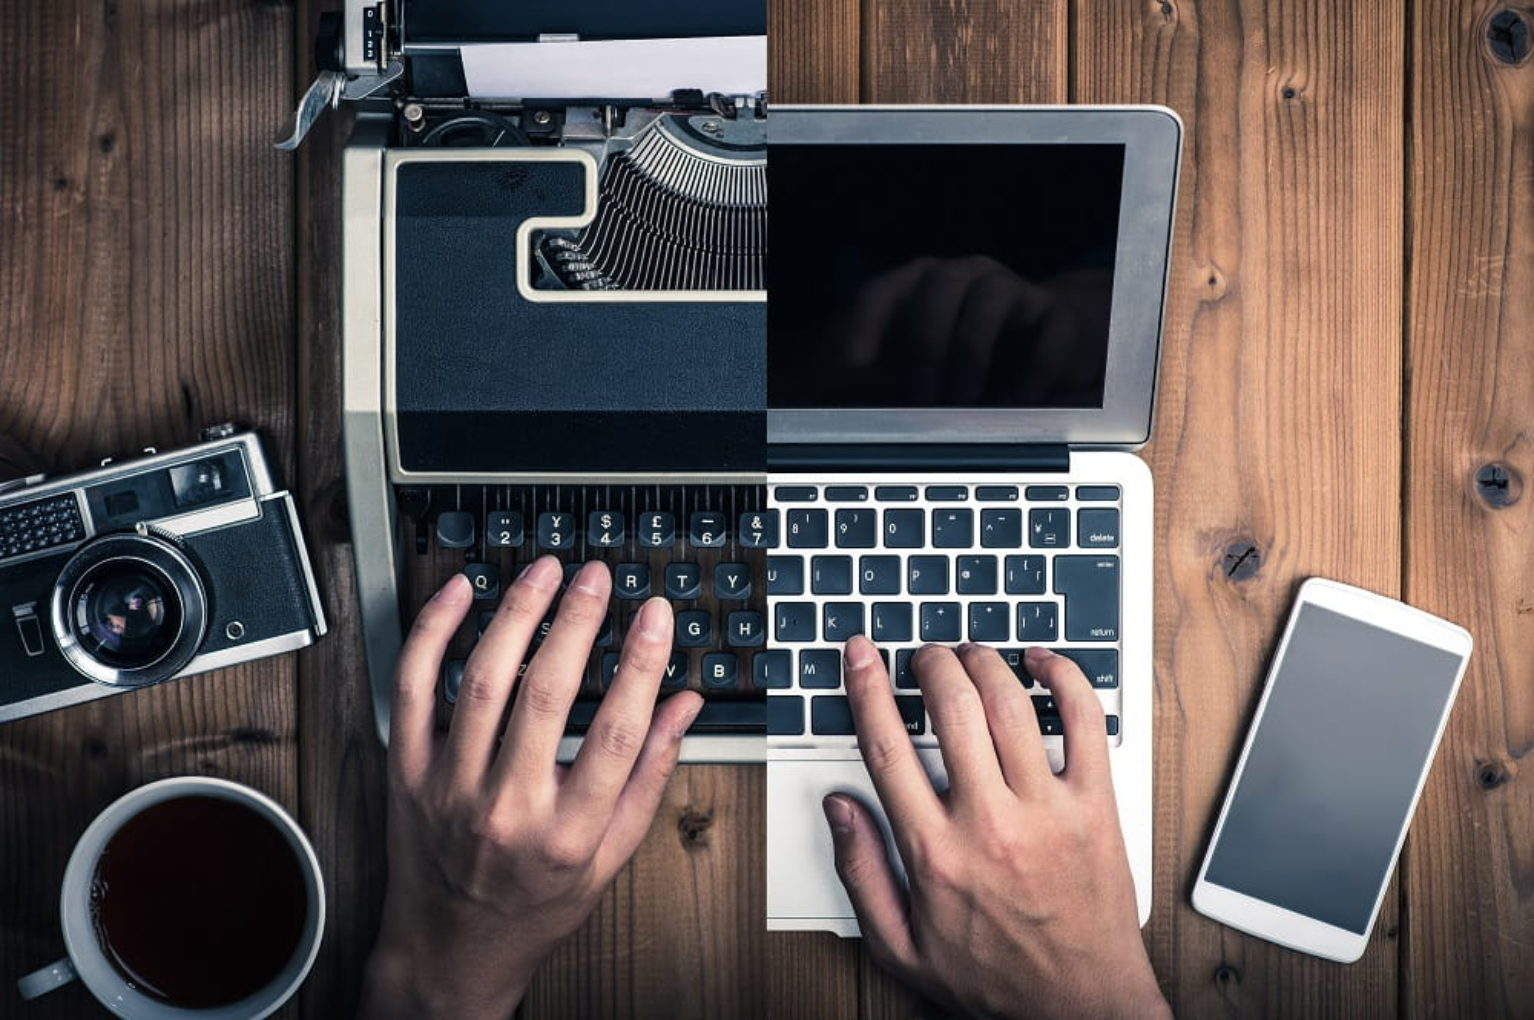
\includegraphics[width=0.75\columnwidth]{immagini/outdated.jpeg}
    \caption{\textit{Obsolete technologies vs modern technologies} - Fonte: \href{https://alfapeople.com/outdated-processes-damage-business-part-1-obsolete-technologies/}{How Outdated Processes Damage Your Business - Alpha People}}
    \label{fig:oldTech}
\end{figure}
\newpage

\subsubsection{Implementazione}
%**************************************************************
\paragraph{VS Code}
L'\acrshort{ide} marchiato Microsoft mi ricorda più degli editor di testo con funzionalità avanzate per interfaccia grafica rispetto ad un ambiente di sviluppo come lo intendo in un accezione più moderna. Ciononostante, tramite l'aggiunta di \textit{plug-in}, riesce a fornire un buon servizio con un consumo estremamente basso di risorse hardware.
Il reparto lo utilizza per lo sviluppo in Angular: personalmente non mi è piaciuta la meccanica di \textit{code completion} rispetto all'offerta dei \textit{competitor} o del fratello maggiore Microsoft Visual Studio\footnote{Personale esperienza con la versione 2011}.
%**************************************************************
\paragraph{IntelliJ IDEA}
Tramite lo strumento sviluppato da JetBrains, ho gestito tutto il processo di \textit{build} delle componenti Micronaut nel \textit{back-end} della piattaforma tramite l'agilissima configurazione dei task tramite \gls{gradle}. Il \textit{tool} è completo, anche rispetto ad altri \textit{framework} e linguaggi e il completamento del codice è gradevolmente farcito con un accesso rapido alla documentazione in fase di consultazione delle opzioni disponibili. Il terminale è ben integrato con una certa autonomia nel lancio dei comandi di build, test, esecuzione e debug. In accessibilità, qualche comportamento da segnalare: alcune \textit{shortcut} non corrispondono al comportamento atteso per convenzione di sistema operativo; è sufficiente però costruirsi una propria configurazione per ovviare a questo problema. Difetto evidente invece è l'utilizzo di risorse (comprensibile vista la gamma di funzionalità offerte) che lo rende difficile da utilizzare con i \textit{device} più datati.
%**************************************************************
\paragraph{WebStorm}
Specializzato in sviluppo web, WebStorm si propone come la versione \textit{light-weight} di IntelliJ IDEA. Posso affermare con sicurezza che è più leggero e snello nell'uso ma allo stesso tempo che non lo è sufficientemente per operare con i dispositivi meno recenti. La \textit{code completion} lavora molto bene sul codice Typescript del \textit{framework} Angular ma, non appena le risorse hardware cominciano a scarseggiare, diventa inutilizzabile.

Nel complesso, i programmi marchiati JetBrains sono molto potenti e di conseguenza richiedono molte risorse.
%**************************************************************
\paragraph{GitLab}
Tramite questo software di controllo di versione, abbiamo inserito il codice all'interno di un \textit{branch} dedicato al mio stage. Da esso, ho creato personalmente diverse ramificazioni per gestire le varie funzionalità in maniera separata, andandole poi ad integrare tramite l'operazione di \textit{merge}. Le funzionalità sono state testate tramite l'ambiente di sviluppo da me riprodotto (spiegato in \S\ref{ssec:docker}) perciò, l'integrazione nel ramo principale è risultata indolore.
%**************************************************************
\subsubsection{Verifica}
%**************************************************************
\paragraph{JUnit}
Tramite questo \textit{framework} è possibile testare anche il codice Java. Nel caso di Bipod, viene usato per controllare le \acrshort{api} implementate in Micronaut. Ogni modifica effettuata al codice \textit{back-end} ha comportato l'aggiornamento del corrispettivo codice di test includendo la verifica delle nuove funzionalità introdotte.
\newpage
%**************************************************************
\paragraph{Protractor}
Durante la formazione iniziale riguardo alle tecnologie, ho effettuato delle prove con il \textit{framework} di \textit{testing} Protractor. Il suo funzionamento è estremamente interessante: permette di definire dei veri e propri casi d'uso indicando l'azione utente che si desidera modellare e il comportamento atteso tramite delle asserzioni.
Purtroppo, confrontandoci con il responsabile, abbiamo constatato la mancanza di risorse temporali per implementare questo tipo di test. Per come sono strutturati i controlli descritti con questo strumento, sarebbe stato estremamente utile modellare i comportamenti cruciali che abbiamo definito durante le revisioni di progettazione.
\begin{figure}[H]
    \centering
    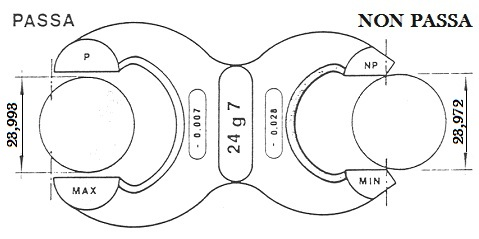
\includegraphics[width=0.65\columnwidth]{immagini/passa-non-passa.jpg}
    \caption{Calibro passa-non passa - Fonte: \href{https://meccanicatecnica.altervista.org/calibri-fissi/}{Calibri fissi - Meccanica Tecnica}}
    \label{fig:passaNonPassa}
\end{figure}
%**************************************************************
\subsection{\gls{solid} \textit{principles}}
Il mio primo approccio a Bipod è avvenuto durante uno dei colloqui precedenti l'inizio dell'attività di stage. Il responsabile, mi ha mostrato il prototipo che era stato creato da un altro studente in precedenza. Una volta che ho avuto l'accesso al codice, ho notato diverse criticità che andavano risolte prima di affrontare il discorso \acrshort{ux}. Le più disturbanti erano la mancanza di strutturazione e l'innesto di componenti effettuato violando i principi \gls{solid}\glsfirstoccur.
C'erano, infatti, alcune elaborazioni riguardanti la \textit{business-logic} all'interno delle componenti grafiche.
Un altro problema era la rappresentazione \textit{back-end} della \textit{business-logic}. \acrshort{json} è un ottimo formato di dati che si comporta bene con JavaScript (per definizione) su cui sono basate molte librerie per la comunicazione su protocollo \acrshort{http}.
Purtroppo, chi ha progettato la partizione \textit{back-end} di inserimento e gestione \acrshort{kpi}, ha deciso di impiegarlo in maniera leggermente inappropriata: dati che logicamente dovevano essere inseriti all'interno di determinati oggetti erano stati serializzati in dizionari \acrshort{json} separati. Inoltre ho notato che venivano impiegati \textit{array} per serializzare oggetti che dovevano avere un nome univoco, introducendo un controllo ulteriore che avrebbe dovuto essere fatto nel momento del salvataggio. Queste criticità minacciano l'integrità e la coerenza fra dati correlati. Una soluzione che ho proposto è quella di sfruttare il vincolo relazionale all'interno del database PostgreSQL per rappresentare tali informazioni e delegarne così l'integrità al \acrshort{dbms}. Il responsabile ha apprezzato questa proposta e ha detto che programmerà un ciclo di restauro \textit{back-end} per risolvere il problema.

Per agevolare questa operazione futura, ho strutturato il mio codice basandomi sulla separazione delle componenti con logica propria e sul rispetto dei principi \gls{solid}.
%**************************************************************
\subsection{\textit{\acrshort{rest}fullnes}}
Nelle due partizioni di software interessate dalla mia attività di stage ho notato che sia internamente, sia durante le comunicazioni fra di loro, avvenivano violazioni dei principi \acrshort{rest}. Ho deciso perciò di far rispettare al codice \textit{front-end} questa convenzione. Inoltre ho creato ex-novo il \textit{service} di comunicazione con il \textit{back-end} e modificato le \acrshort{api} in quest'ultimo sfruttando le annotazioni parametrizzando le chiamate con gli identificatori degli oggetti di interesse. Ho dovuto anche modificare le intestazioni e annotazioni di quasi tutti i metodi sviluppati su Micronaut per utilizzare le corrette chiamate \acrshort{http} in base all'operazione di interesse.
\vspace{45pt}
\begin{figure}[H]
    \centering
    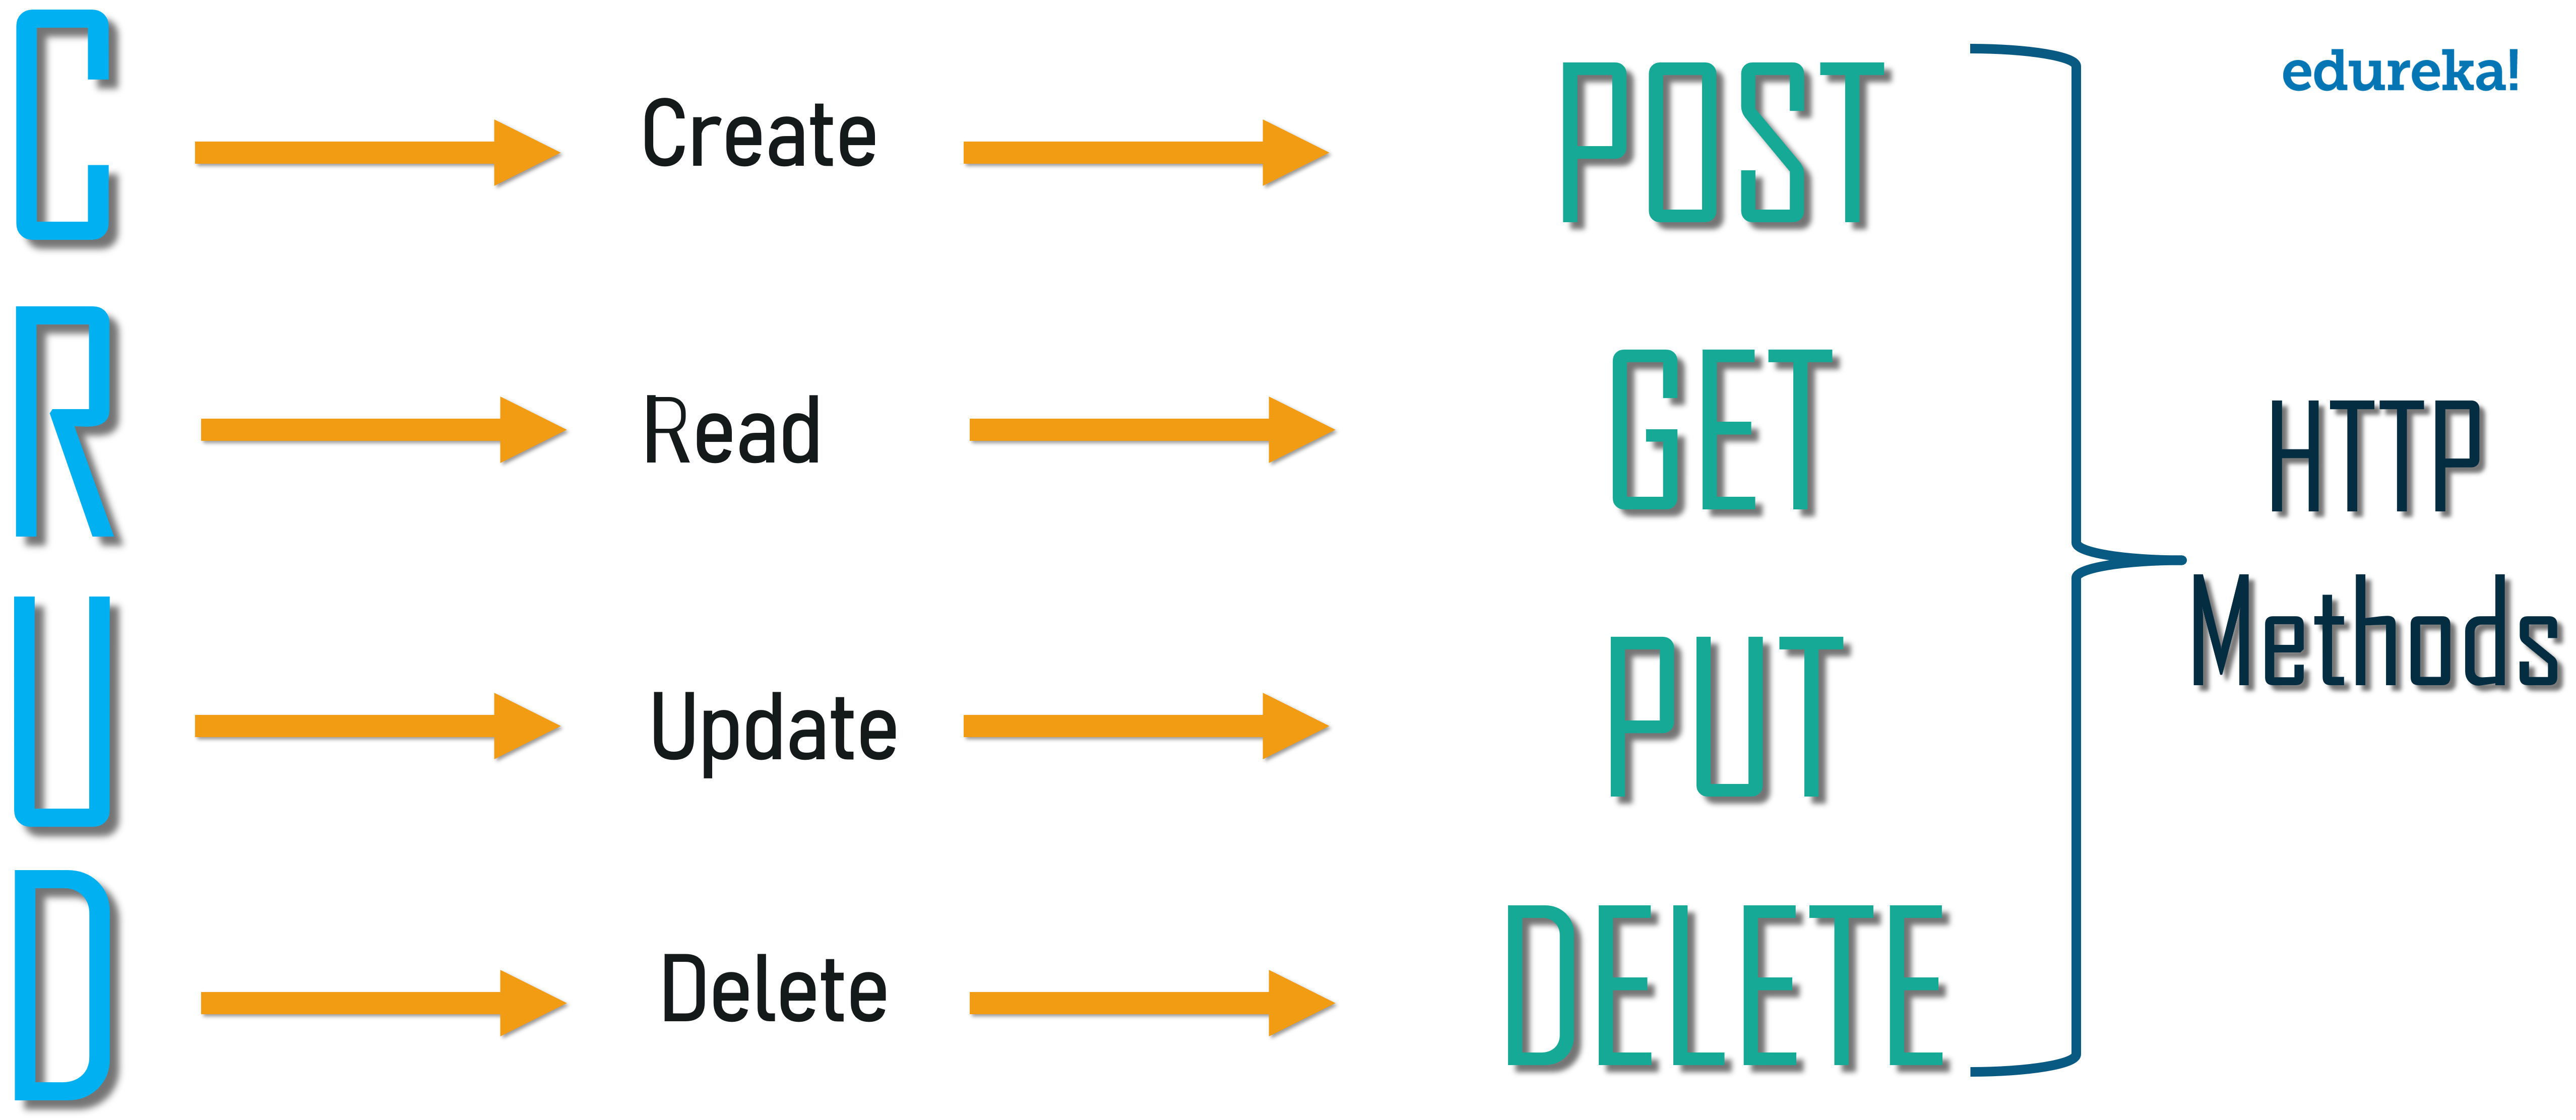
\includegraphics[width=0.90\columnwidth]{immagini/crudToRest.png}
    \caption{CRUD to REST - Fonte: \href{https://www.edureka.co/blog/what-is-rest-api/}{What is REST API? - Edureka}}
    \label{fig:crudToRest}
\end{figure}
\vspace{45pt}
%**************************************************************
\subsection{Riuso del codice}
I file HTML impiegati per descrivere le \textit{form} di inserimento di termini e \acrshort{kpi} sono interpretati da Angular come veri e propri \textit{template}. Questo significa che sono a tutti gli effetti dei modelli di interfaccia grafica: ho deciso perciò di implementare le funzionalità di modifica di termini e \acrshort{kpi} sfruttando l'ereditarietà. Fra una \textit{form} di inserimento e una di modifica dello stesso componente, non cambiano ne le politiche di validazione della struttura del dato e nemmeno le regole di coerenza interne all'oggetto che sto definendo/modificando. Ho implementato perciò nella classe base il comportamento atteso dall'operazione di aggiunta elementi, effettuando l'\textit{override} dei metodi per ottenere il comportamento di modifica nella classe derivata.
\newpage
%**************************************************************
\subsection{Esperienza utente}
Parte delle funzionalità di gestione dei \acrshort{kpi} era già stato fornito nelle versioni precedenti della piattaforma. Questo mi ha permesso di capire più velocemente la meccanica di base di tali operazioni. Il core della mia attività di stage è stata la valutazione delle esigenze utente durante tutti gli scenari di utilizzo possibili.

La difficoltà principale nell'effettuare tale operazione è stata riuscire ad immaginarsi quale sarebbero potute essere le possibili interazioni con un software di cui non avevo ancora fatto mia l'utilità. Questo era dovuto anche alla mancante assimilazione dei concetti di \textit{process mining} che dovevano ancora prendere una forma definita nella mia testa.
Provando ad utilizzare l'interfaccia grafica di Bipod, ho individuato delle criticità che si sono rivelate base solida per definire l'esperienza utente nella gestione degli indicatori di performance.
Per quanto riguarda la parte di \textit{dashboard} e di visualizzazione dei grafi di processo, ho dovuto confrontarmi con il responsabile per riuscire ad inquadrare il problema.

Le peculiarità che ho voluto concretizzare nell'\acrshort{ux} sono le seguenti:
\begin{itemize}
    \item Fornitura di un sistema di ricerca di \acrshort{kpi} intuitivo e rapidamente accessibile;
    \item Disposizione delle componenti ampia e organizzata secondo una logica derivata dagli scenari descritti che comporta un accesso rapido alle informazioni;
    \item Facilitazione del riuso dei dati già inseriti per velocizzare operazioni iterative all'utente;
    \item Estensibilità delle informazioni tramite personalizzazione di alcuni elementi come le unità di misura;
    \item Informazioni tramite impatto grafico già all'interno delle viste;
    \item Selezione delle informazioni da mostrare al primo impatto;
    \item Sistema di \textit{completion} dei parametri che l'utente deve inserire ovunque possibile;
    \item Sistema di collocazione spaziale dei componenti grafici della \textit{dashboard} tramite meccanismo \textit{drag and drop};
    \item Gestione degli intervalli temporali avanzata, personalizzabile e, sopratutto, intuitiva.
\end{itemize}
%**************************************************************
\subsection{Versioni software}
Durante l'attività di implementazione, ho avuto difficoltà a concretizzare in Bipod, una funzionalità dimostrata tramite \acrshort{poc} al responsabile. Mi sono confrontato con il tutor a riguardo e ho scoperto che la versione di Angular in uso sulla piattaforma era obsoleta e che il dimostrativo che avevo creato era invece basato su una versione recente da me installata in locale. Consultando infatti la documentazione del produttore per la specifica versione, ho scoperto che tale funzionalità non era ancora stata sviluppata. Inoltre, la nomenclatura di un evento e del suo tipo, erano state cambiate nella versione nuova.
Ho fatto una rapida valutazione di fattibilità sul passaggio alla nuova versione provando ad aggiornarla. L'operazione ha introdotto diversi problemi di compatibilità, difficili da affrontare tutti insieme. Ho perciò capito l'importanza di aggiornare in tempo utile le versioni software: quando possibile va verificata frequentemente la fattibilità e vanno consultati i \textit{changelog} per controllare se alcune funzionalità sono state deprecate o se sono cambiati i requisiti di alcune librerie o pacchetti.
%**************************************************************
\section{Risultati raggiunti}
%**************************************************************
\subsection{Obiettivi dell'attività di stage}
Gli obiettivi, che ho definito assieme al responsabile, del mio progetto di stage erano diversi, alcuni più sfidanti, altri meno.
Sono elencati nella seguente tabella, categorizzati secondo la nomenclatura:
\begin{center}
    O<tipo><progressivo>
\end{center}
dove
\begin{itemize}
    \item <tipo> indica la tipologia che li discrimina fra O - \textit{obbligatori} e F - \textit{facoltativi};
    \item <progressivo> è un numero progressivo.
\end{itemize}
\begin{table}[H]
    \centering
    \begin{tabular}{|m{0.09\textwidth}|m{0.76\textwidth}|}
        \hline
        \textbf{Codice} & \textbf{Descrizione} \\ \hline
        OO1 & Inquadramento del problema: stesura di un documento di specifica del problema \\ \hline
        OO2 & Analisi di casi d’uso e requisiti\\ \hline
        OO3 & Progettazione dell’interfaccia per ciascuna delle funzionalità indicate con eventuali mock-up \\ \hline
        OO4 & Sviluppo del frontend di gestione dei KPI \\ \hline
        OO5 & Documentazione: descrizione degli strumenti e delle tecniche utilizzate, descrizione dell’architettura del sistema, documentazione del progetto per lo sviluppatore e dei passi necessari per installare ed eseguire il tutto \\ \hline
        OF1 & Analisi, progettazione e sviluppo della dashboard personalizzabile per il manager \\ \hline
        OF2 & Analisi, progettazione e sviluppo di un modulo per la rappresentazione della value stream \\ \hline
        OF3 & Gestione del point-and-click sul processo per eventuali arricchimenti dello schema di processo \\ \hline
        OF4 & Gestione permessi utenti \\ \hline
    \end{tabular}
    \caption{Tabella degli obbiettivi dell'attività di stage}
    \label{tab:obiettivi}
\end{table}
Da questi obiettivi discende a cascata il seguente tracciamento dei requisiti indicati in \S\ref{sec:aspettative}
\begin{table}[H]
    \centering
    \begin{tabular}{|c|m{0.8\textwidth}|}
    \hline
        \textbf{Obiettivo} & \textbf{Requisiti da soddisfare} \\ \hline
        OO4 & RO2, RO2.1, RO2.2, RO2.2.1, RO2.2.2, RO2.2.3, RO2.3, RO3, RO3.1, RO3.2, RO3.3 \\ \hline
        OF1 & RF1, RF1.1, RF1.1.1, RF1.1.2, RF1.1.3, RF1.1.4 \\ \hline
        OF2 & RF3, RF3.1, RF3.2 \\ \hline
        OF3 & RF3.2 \\ \hline
        OF4 & RO2.2.3 \\ \hline
    \end{tabular}
    \caption{Tracciamento dei requisiti rispetto gli obiettivi}
    \label{tab:tracciamento}
\end{table}
\newpage
\subsection{Raggiungimento degli obiettivi}
A termine del periodo di stage, ho effettuato, insieme al responsabile, la verifica dei requisiti presentati in \S\ref{sec:aspettative}. Il risultato è il seguente:
\begin{table}[H]
    \centering
    \begin{tabular}{|c|c|}
    \hline
        \textbf{Requisito} & {Soddisfacimento} \\
        \rowcolor{green!15} RO1 & Soddisfatto \\ \hline
        \rowcolor{green!15} RO2 & Soddisfatto \\  \hline
        \rowcolor{green!15} RO2.1 & Soddisfatto \\  \hline
        \rowcolor{green!15} RO2.2 & Soddisfatto \\  \hline
        \rowcolor{green!15} RO2.2.1 & Soddisfatto \\  \hline
        \rowcolor{green!15} RO2.2.2 & Soddisfatto \\  \hline
        \rowcolor{green!15} RO2.2.3 & Soddisfatto \\  \hline
        \rowcolor{green!15} RO2.3 & Soddisfatto \\  \hline
        \rowcolor{green!15} RO3 & Soddisfatto \\  \hline
        \rowcolor{green!15} RO3.1 & Soddisfatto \\  \hline
        \rowcolor{green!15} RO3.2 & Soddisfatto \\  \hline
        \rowcolor{green!15} RO3.3 & Soddisfatto \\  \hline
        \rowcolor{red!15} RF1 & Non soddisfatto \\ \hline
        \rowcolor{red!15} RF1.1 & Non soddisfatto \\ \hline
        \rowcolor{red!15} RF1.1.1 & Non soddisfatto \\ \hline
        \rowcolor{red!15} RF1.1.2 & Non soddisfatto \\ \hline
        \rowcolor{red!15} RF1.1.3 & Non soddisfatto \\ \hline
        \rowcolor{red!15} RF1.1.4 & Non soddisfatto \\ \hline
        \rowcolor{red!15} RF2 & Non soddisfatto \\ \hline
        \rowcolor{red!15} RF3 & Non soddisfatto \\ \hline
        \rowcolor{red!15} RF3.1 & Non soddisfatto \\ \hline
        \rowcolor{red!15} RF3.2 & Non soddisfatto \\ \hline
        \rowcolor{red!15} RF3.3 & Non soddisfatto \\ \hline
    \end{tabular}
    \caption{Caption}
    \label{tab:my_label}
\end{table}

Di conseguenza, il livello di raggiungimento degli obiettivi, non è stato quello da me desiderato ma comunque sufficiente.
Ecco lo stato di raggiungimento degli stessi assieme al prodotto che lo ha permesso:

\begin{table}[H]
    \centering
    \begin{tabular}{|m{0.08\textwidth}|m{0.20\textwidth}|m{0.72\textwidth}|}
    \hline
        \textbf{Codice} & \textbf{Raggiungimento} & \textbf{Prodotto} \\ \hline
        \rowcolor{green!15}
        OO1 & Raggiunto & Nota Evernote "Inquadramento stage Bettarello Alessio" \\ \hline
        \rowcolor{green!15}
        OO2 & Raggiunto & Documento "Analisi dei requisiti" \\ \hline
        \rowcolor{green!15}
        OO3 & Raggiunto & Documento Evernote "Specifiche tecniche" \\ \hline
        \rowcolor{green!15}
        OO4 & Raggiunto & Codice sorgente all'interno del \textit{repository} \\ \hline
        \rowcolor{green!15}
        OO5 & Raggiunto & Documento "Specifiche tecniche" e codice sorgente all'interno del
        \textit{repository} \\ \hline
        \rowcolor{orange!15}
        OF1 & Parzialmente & Analisi presente in "Analisi dei requisiti" \\ \hline
        \rowcolor{red!15}
        OF2 & Non raggiunto & \\ \hline
        \rowcolor{red!15}
        OF3 & Non raggiunto & \\ \hline
        \rowcolor{red!15}
        OF4 & Non raggiunto & \\ \hline
    \end{tabular}
    \caption{Livello di soddisfacimento degli obiettivi di stage}
    \label{tab:goalObiettivi}
\end{table}


%**************************************************************
\subsection{Analisi dei requisiti}
Il primo e,a mio parere, più importante prodotto dell'attività di stage, è l'analisi dei requisiti.
\'E lo strumento più efficace per esprimere la base dell'\acrshort{ux} che si vuole fornire.

Per questioni di completezza e coerenza, l'ho effettuata su tutte le funzionalità che la piattaforma deve fornire.
Una volta ultimata l'analisi, i macro-scenari individuati erano i seguenti:
\begin{itemize}
    \item Autenticazione
    \item Visualizzazione \textit{dashboard}
    \item Visualizzazione \acrshort{kpi} in osservazione
    \item Creazione \acrshort{kpi}
    \item Modifica \acrshort{kpi}
    \item Creazione termini
    \item Modifica termini
\end{itemize}

Di ognuno di essi ho analizzato il dettaglio come descritto in \S\ref{ssec:diagrams}.
Per aumentare la precisione sono state inserite le caratteristiche fondamentali degli scenari indicando anche pre e post condizioni.
Ho poi definito a cascata a i requisiti a cui la piattaforma deve rispondere facilitando in seguito la verifica dell'operato del gruppo. Parte di essi è riportato in \S\ref{sec:aspettative}

Il documento è composto dall'analisi di 34 casi d'uso che hanno introdotto 86 requisiti. Di questi, ne abbiamo soddisfatti 63 ovvero una percentuale del 73\%.
\vspace{50pt}
\begin{figure}[H]
    \centering
    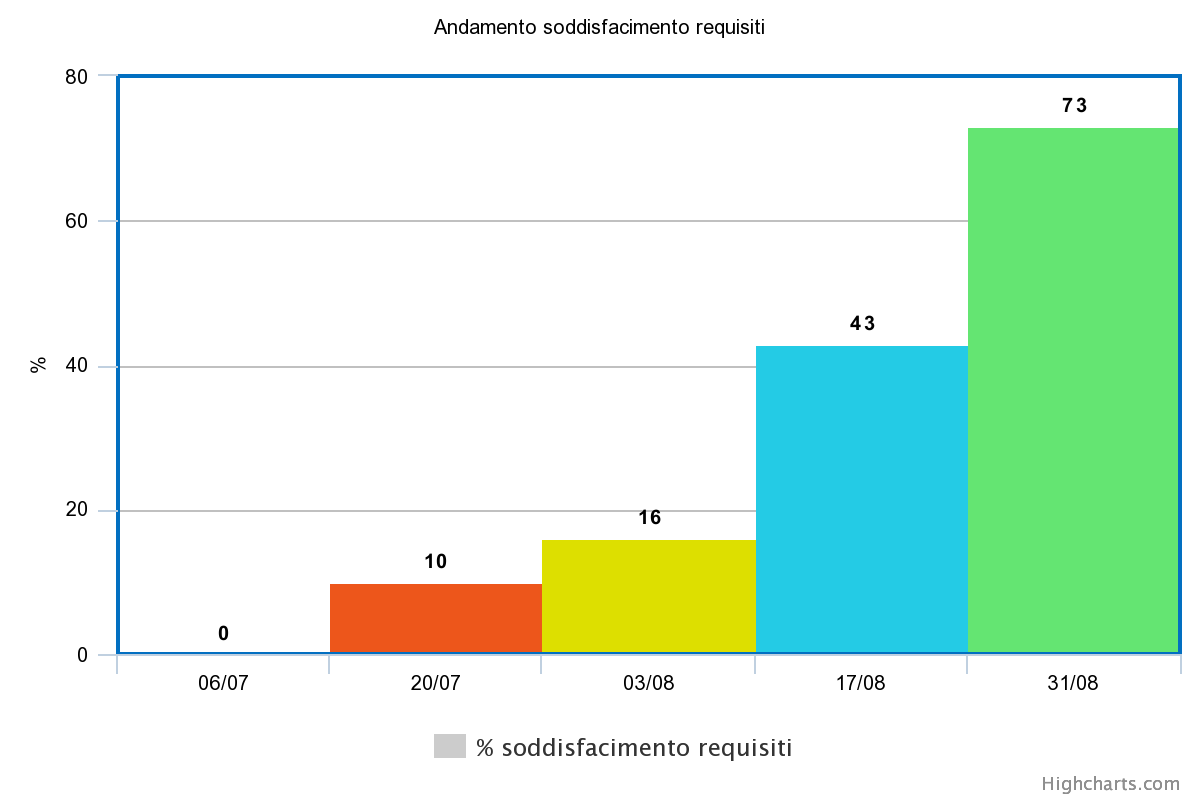
\includegraphics[width=0.65\columnwidth]{immagini/chart.png}
    \caption{Andamento soddisfacimento dei requisiti}
    \label{fig:reqChart}
\end{figure}
\newpage
%**************************************************************
\subsection{Diario delle attività}
L'utilità che ho percepito di questo documento condiviso è molteplice: per prima cosa aiuta a capire le attività che eseguo portino al giusto traguardo; inoltre aiuta me e i colleghi a tenere traccia delle scelte tecniche intraprese per ovviare agli imprevisti sorti durante il percorso. L'ho redatto giorno per giorno indicando in maniera essenziale cosa è stato fatto e in maniera più prolissa, qualora abbia fatto analisi critiche.
%**************************************************************
\subsection{Specifiche tecniche}
Qualora, nel corso del progetto, io abbia dovuto effettuare scelte tecniche da intraprendere, ho riportato le informazioni tecniche e le motivazioni delle mie scelte in una nota Evernote chiamata "Specifiche tecniche".Essendo presente nel taccuino relativo allo stage, essa è condivisa e facilmente fruibile dal responsabile.
Le scelte tecniche più significative sono le seguenti:
\begin{itemize}
    \item Eliminazione delle vecchie componenti in favore di maggiore separazione;
    \item Gestione progettuale tramite \acrshort{poc} e \textit{mock} dei \textit{service} invece che con \textit{mock-up} grafici;
    \item Scelta di replicare i controlli sui dati \textit{back-end} anche nelle corrispettive chiamate \textit{front-end};
    \item Scelta dell'utilizzo della sorgente dati Material Data Table per la visualizzazione tabulare al posto di rappresentazione tabulare HTML classica;
    \item Aggiunta, nel modello dei dati relativi ai \acrshort{kpi}, delle informazioni relative all'unità di misura
    \item Scelta del meccanismo di selezione date per \textit{sliding window} basato su operazioni di resto della divisione intera
    \item Modifica delle \acrshort{api} \textit{back-end} per rispettare i principi \acrshort{rest}
\end{itemize}
\newpage
%**************************************************************
\subsection{Codice sorgente}
Ho effettuato la concretizzazione dello studio dell'\acrshort{ux} di Bipod tramite la stesura di codice TypeScript e Java. Tutto ciò che ho implementato risiede nel \textit{repository} aziendale ed è perciò accessibile da tutto il reparto. Ogni versione del codice che ho caricato, contiene incrementi significativi che evidenziano perciò quali modifiche ho effettuato per aggiungere una determinata funzionalità. Il prodotto codice sorgente non è perciò da intendersi dal lettore come monade ma come successione di \gls{commit} che mi ha portato al risultato ottenuto.
Nella tabella seguente ho indicato alcune rilevazioni effettuate sul codice:
\begin{table}[H]
    \centering
    \begin{tabular}{|c|c|}
    \hline
        \# commit effettuati & 40 \\ \hline
        \# File di codice modificati & 65 \\ \hline
        \# File di codice aggiunti & 17 \\ \hline
        \# Righe modificate & 6632 \\ \hline
        \ Media copertura \textit{docstrings} & 92.94\% \\ \hline
        \# Ore di codifica & 88 \\ \hline
    \end{tabular}
    \caption{Dati sul codice}
    \label{tab:codeData}
\end{table}
\begin{figure}[H]
    \centering
    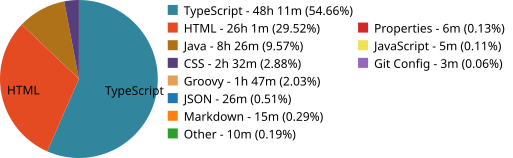
\includegraphics[width=0.9\columnwidth]{immagini/linguaggi.png}
    \caption{Suddivisione oraria per linguaggio (tempo di digitazione)}
    \label{fig:languages}
\end{figure}
%**************************************************************             % Modalità di svolgimento dello stage
% !TEX encoding = UTF-8
% !TEX TS-program = pdflatex
% !TEX root = ../tesi.tex

%**************************************************************
\chapter{Indici di prestazione dello stage}
\label{cap:performance-stage}
%**************************************************************

\section{Come si è svolta l'attività di stage}
%**************************************************************
\subsection{Andamento}
La sezione espone cosa ho percepito nei cambiamenti di ritmo fra i lenti momenti di confronto e le veloci realizzazioni di POC e codice
%**************************************************************
\subsection{Aspettativa vs realtà: il completamento degli obiettivi}
Mostra come la sicurezza di riuscire a soddisfare tutti requisiti, si sia tramutata poi in cura rispetto a quelli che erano gli obbligatori per portare al raggiungimento della finalità dello stage ovvero quello di incremento qualitativo del lavoro svolto
%**************************************************************
\subsection{Cicli di sviluppo: Micro vs Macro}
Mostra come confrontandoci all'interno del team, siamo passati da un piano di progetto "a ciclo unico" a diversi cicli di sviluppo via via che si formalizzavano i requisiti e veniva verificata la fattibilità di ogni singola parte

%**************************************************************
\section{Analisi di profitto}
%**************************************************************
\subsection{Teamworking informatico}
Sezione in cui parlo della prima esperienza di teamworking in ambito informatico (fuori dal contesto scolastico) e di cosa mi ha arrichito
%**************************************************************
\subsection{Il mio contributo al team}
Sezione in cui espongo cosa delle mie conoscenze preliminari ho prestato al team e perché sono state apprezzate
%**************************************************************
\subsection{Un corretto way of thinking dello studente di Informatica Unipd}
La mia opinione sulla giusta strada per guadagnare il massimo da questo corso di laurea.             % Indici di prestazione dello stage

%**************************************************************
% Materiale finale
%**************************************************************
\backmatter
\printglossary[type=acronym, title={Acronimi}]
\printglossary[type=main,title={Glossario}]
% !TEX encoding = UTF-8
% !TEX TS-program = pdflatex
% !TEX root = ../tesi.tex

%**************************************************************
% Bibliografia
%**************************************************************

\cleardoublepage
\chapter{Bibliografia}

\nocite{*}
% Stampa i riferimenti bibliografici
\printbibliography[heading=subbibliography,title={Riferimenti bibliografici},type=book]

% Stampa i siti web consultati
%\printbibliography[heading=subbibliography,title={Siti web consultati},type=online]


\end{document}
